\documentclass[twoside]{book}

% Packages required by doxygen
\usepackage{fixltx2e}
\usepackage{calc}
\usepackage{doxygen}
\usepackage[export]{adjustbox} % also loads graphicx
\usepackage{graphicx}
\usepackage[utf8]{inputenc}
\usepackage{makeidx}
\usepackage{multicol}
\usepackage{multirow}
\PassOptionsToPackage{warn}{textcomp}
\usepackage{textcomp}
\usepackage[nointegrals]{wasysym}
\usepackage[table]{xcolor}

% Font selection
\usepackage[T1]{fontenc}
\usepackage[scaled=.90]{helvet}
\usepackage{courier}
\usepackage{amssymb}
\usepackage{sectsty}
\renewcommand{\familydefault}{\sfdefault}
\allsectionsfont{%
  \fontseries{bc}\selectfont%
  \color{darkgray}%
}
\renewcommand{\DoxyLabelFont}{%
  \fontseries{bc}\selectfont%
  \color{darkgray}%
}
\newcommand{\+}{\discretionary{\mbox{\scriptsize$\hookleftarrow$}}{}{}}

% Page & text layout
\usepackage{geometry}
\geometry{%
  a4paper,%
  top=2.5cm,%
  bottom=2.5cm,%
  left=2.5cm,%
  right=2.5cm%
}
\tolerance=750
\hfuzz=15pt
\hbadness=750
\setlength{\emergencystretch}{15pt}
\setlength{\parindent}{0cm}
\setlength{\parskip}{3ex plus 2ex minus 2ex}
\makeatletter
\renewcommand{\paragraph}{%
  \@startsection{paragraph}{4}{0ex}{-1.0ex}{1.0ex}{%
    \normalfont\normalsize\bfseries\SS@parafont%
  }%
}
\renewcommand{\subparagraph}{%
  \@startsection{subparagraph}{5}{0ex}{-1.0ex}{1.0ex}{%
    \normalfont\normalsize\bfseries\SS@subparafont%
  }%
}
\makeatother

% Headers & footers
\usepackage{fancyhdr}
\pagestyle{fancyplain}
\fancyhead[LE]{\fancyplain{}{\bfseries\thepage}}
\fancyhead[CE]{\fancyplain{}{}}
\fancyhead[RE]{\fancyplain{}{\bfseries\leftmark}}
\fancyhead[LO]{\fancyplain{}{\bfseries\rightmark}}
\fancyhead[CO]{\fancyplain{}{}}
\fancyhead[RO]{\fancyplain{}{\bfseries\thepage}}
\fancyfoot[LE]{\fancyplain{}{}}
\fancyfoot[CE]{\fancyplain{}{}}
\fancyfoot[RE]{\fancyplain{}{\bfseries\scriptsize Generated by Doxygen }}
\fancyfoot[LO]{\fancyplain{}{\bfseries\scriptsize Generated by Doxygen }}
\fancyfoot[CO]{\fancyplain{}{}}
\fancyfoot[RO]{\fancyplain{}{}}
\renewcommand{\footrulewidth}{0.4pt}
\renewcommand{\chaptermark}[1]{%
  \markboth{#1}{}%
}
\renewcommand{\sectionmark}[1]{%
  \markright{\thesection\ #1}%
}

% Indices & bibliography
\usepackage{natbib}
\usepackage[titles]{tocloft}
\setcounter{tocdepth}{3}
\setcounter{secnumdepth}{5}
\makeindex

% Hyperlinks (required, but should be loaded last)
\usepackage{ifpdf}
\ifpdf
  \usepackage[pdftex,pagebackref=true]{hyperref}
\else
  \usepackage[ps2pdf,pagebackref=true]{hyperref}
\fi
\hypersetup{%
  colorlinks=true,%
  linkcolor=blue,%
  citecolor=blue,%
  unicode%
}

% Custom commands
\newcommand{\clearemptydoublepage}{%
  \newpage{\pagestyle{empty}\cleardoublepage}%
}

\usepackage{caption}
\captionsetup{labelsep=space,justification=centering,font={bf},singlelinecheck=off,skip=4pt,position=top}

%===== C O N T E N T S =====

\begin{document}

% Titlepage & ToC
\hypersetup{pageanchor=false,
             bookmarksnumbered=true,
             pdfencoding=unicode
            }
\pagenumbering{roman}
\begin{titlepage}
\vspace*{7cm}
\begin{center}%
{\Large Lift project }\\
\vspace*{1cm}
{\large Generated by Doxygen 1.8.11}\\
\end{center}
\end{titlepage}
\clearemptydoublepage
\tableofcontents
\clearemptydoublepage
\pagenumbering{arabic}
\hypersetup{pageanchor=true}

%--- Begin generated contents ---
\chapter{File Index}
\section{File List}
Here is a list of all documented files with brief descriptions\+:\begin{DoxyCompactList}
\item\contentsline{section}{source/{\bfseries channels.\+h} }{\pageref{channels_8h}}{}
\item\contentsline{section}{source/{\bfseries door.\+c} }{\pageref{door_8c}}{}
\item\contentsline{section}{source/{\bfseries door.\+h} }{\pageref{door_8h}}{}
\item\contentsline{section}{source/{\bfseries elev.\+c} }{\pageref{elev_8c}}{}
\item\contentsline{section}{source/{\bfseries elev.\+h} }{\pageref{elev_8h}}{}
\item\contentsline{section}{source/{\bfseries F\+S\+M.\+c} }{\pageref{FSM_8c}}{}
\item\contentsline{section}{source/{\bfseries F\+S\+M.\+h} }{\pageref{FSM_8h}}{}
\item\contentsline{section}{source/{\bfseries io.\+c} }{\pageref{io_8c}}{}
\item\contentsline{section}{source/{\bfseries io.\+h} }{\pageref{io_8h}}{}
\item\contentsline{section}{source/{\bfseries lift\+Movement.\+c} }{\pageref{liftMovement_8c}}{}
\item\contentsline{section}{source/{\bfseries lift\+Movement.\+h} }{\pageref{liftMovement_8h}}{}
\item\contentsline{section}{source/\hyperlink{main_8c}{main.\+c} \\*The main file, it does what main files usually does }{\pageref{main_8c}}{}
\item\contentsline{section}{source/{\bfseries order.\+c} }{\pageref{order_8c}}{}
\item\contentsline{section}{source/{\bfseries order.\+h} }{\pageref{order_8h}}{}
\item\contentsline{section}{source/{\bfseries stop.\+c} }{\pageref{stop_8c}}{}
\item\contentsline{section}{source/{\bfseries stop.\+h} }{\pageref{stop_8h}}{}
\item\contentsline{section}{source/{\bfseries utility.\+h} }{\pageref{utility_8h}}{}
\end{DoxyCompactList}

\chapter{File Documentation}
\hypertarget{channels_8h}{}\section{source/channels.h File Reference}
\label{channels_8h}\index{source/channels.\+h@{source/channels.\+h}}


Channels.  


This graph shows which files directly or indirectly include this file\+:\nopagebreak
\begin{figure}[H]
\begin{center}
\leavevmode
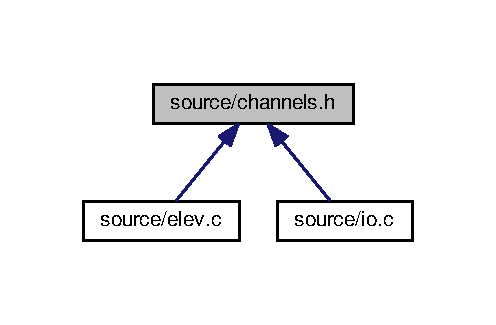
\includegraphics[width=238pt]{channels_8h__dep__incl}
\end{center}
\end{figure}
\subsection*{Macros}
\begin{DoxyCompactItemize}
\item 
\#define {\bfseries P\+O\+R\+T4}~3\hypertarget{channels_8h_ad5a54f368997d8ae4f84a1e2fad533f4}{}\label{channels_8h_ad5a54f368997d8ae4f84a1e2fad533f4}

\item 
\#define {\bfseries O\+B\+S\+T\+R\+U\+C\+T\+I\+ON}~(0x300+23)\hypertarget{channels_8h_a2409f02d98d288f64712887bd13b853e}{}\label{channels_8h_a2409f02d98d288f64712887bd13b853e}

\item 
\#define {\bfseries S\+T\+OP}~(0x300+22)\hypertarget{channels_8h_ae19b6bb2940d2fbe0a79852b070eeafd}{}\label{channels_8h_ae19b6bb2940d2fbe0a79852b070eeafd}

\item 
\#define {\bfseries B\+U\+T\+T\+O\+N\+\_\+\+C\+O\+M\+M\+A\+N\+D1}~(0x300+21)\hypertarget{channels_8h_a1a22e01173ae543c7350d23af9099083}{}\label{channels_8h_a1a22e01173ae543c7350d23af9099083}

\item 
\#define {\bfseries B\+U\+T\+T\+O\+N\+\_\+\+C\+O\+M\+M\+A\+N\+D2}~(0x300+20)\hypertarget{channels_8h_a8f3d02fddfb1ecd5227eca135f19ebd6}{}\label{channels_8h_a8f3d02fddfb1ecd5227eca135f19ebd6}

\item 
\#define {\bfseries B\+U\+T\+T\+O\+N\+\_\+\+C\+O\+M\+M\+A\+N\+D3}~(0x300+19)\hypertarget{channels_8h_a82aab21b1b50d554effcf8b26576b388}{}\label{channels_8h_a82aab21b1b50d554effcf8b26576b388}

\item 
\#define {\bfseries B\+U\+T\+T\+O\+N\+\_\+\+C\+O\+M\+M\+A\+N\+D4}~(0x300+18)\hypertarget{channels_8h_add9ae7df96dfd4ad569d3b703023187d}{}\label{channels_8h_add9ae7df96dfd4ad569d3b703023187d}

\item 
\#define {\bfseries B\+U\+T\+T\+O\+N\+\_\+\+U\+P1}~(0x300+17)\hypertarget{channels_8h_a7236f6ea90139248afabe014632c3cec}{}\label{channels_8h_a7236f6ea90139248afabe014632c3cec}

\item 
\#define {\bfseries B\+U\+T\+T\+O\+N\+\_\+\+U\+P2}~(0x300+16)\hypertarget{channels_8h_a3a95d31cf2002937c921bbd85590bc7a}{}\label{channels_8h_a3a95d31cf2002937c921bbd85590bc7a}

\item 
\#define {\bfseries P\+O\+R\+T1}~2\hypertarget{channels_8h_a83b698b796fa8d1625536439f28ea575}{}\label{channels_8h_a83b698b796fa8d1625536439f28ea575}

\item 
\#define {\bfseries B\+U\+T\+T\+O\+N\+\_\+\+D\+O\+W\+N2}~(0x200+0)\hypertarget{channels_8h_a63a7b9d9d7c23325d4171292d596fa11}{}\label{channels_8h_a63a7b9d9d7c23325d4171292d596fa11}

\item 
\#define {\bfseries B\+U\+T\+T\+O\+N\+\_\+\+U\+P3}~(0x200+1)\hypertarget{channels_8h_aa6b5917715e012cf21e3a89fb7c93e2d}{}\label{channels_8h_aa6b5917715e012cf21e3a89fb7c93e2d}

\item 
\#define {\bfseries B\+U\+T\+T\+O\+N\+\_\+\+D\+O\+W\+N3}~(0x200+2)\hypertarget{channels_8h_ab423174da71ed0d6b083cd8d71f54617}{}\label{channels_8h_ab423174da71ed0d6b083cd8d71f54617}

\item 
\#define {\bfseries B\+U\+T\+T\+O\+N\+\_\+\+D\+O\+W\+N4}~(0x200+3)\hypertarget{channels_8h_a7e1266fcb6843826718edec0222b1e49}{}\label{channels_8h_a7e1266fcb6843826718edec0222b1e49}

\item 
\#define {\bfseries S\+E\+N\+S\+O\+R\+\_\+\+F\+L\+O\+O\+R1}~(0x200+4)\hypertarget{channels_8h_a5ae95fe4e1273653467895d5e7c39377}{}\label{channels_8h_a5ae95fe4e1273653467895d5e7c39377}

\item 
\#define {\bfseries S\+E\+N\+S\+O\+R\+\_\+\+F\+L\+O\+O\+R2}~(0x200+5)\hypertarget{channels_8h_ab9e1c393bf2c51d65ed0a132af8321d3}{}\label{channels_8h_ab9e1c393bf2c51d65ed0a132af8321d3}

\item 
\#define {\bfseries S\+E\+N\+S\+O\+R\+\_\+\+F\+L\+O\+O\+R3}~(0x200+6)\hypertarget{channels_8h_a65904322d022513386fea3bcb9a8b524}{}\label{channels_8h_a65904322d022513386fea3bcb9a8b524}

\item 
\#define {\bfseries S\+E\+N\+S\+O\+R\+\_\+\+F\+L\+O\+O\+R4}~(0x200+7)\hypertarget{channels_8h_a6a8d30abdce8780479ac7f0677200074}{}\label{channels_8h_a6a8d30abdce8780479ac7f0677200074}

\item 
\#define {\bfseries P\+O\+R\+T3}~3\hypertarget{channels_8h_ad906b7f6a811f1f02b5eb04cbe1bc89b}{}\label{channels_8h_ad906b7f6a811f1f02b5eb04cbe1bc89b}

\item 
\#define {\bfseries M\+O\+T\+O\+R\+D\+IR}~(0x300+15)\hypertarget{channels_8h_aaa316c7fc13ca7b9b4229af3f9832a7d}{}\label{channels_8h_aaa316c7fc13ca7b9b4229af3f9832a7d}

\item 
\#define {\bfseries L\+I\+G\+H\+T\+\_\+\+S\+T\+OP}~(0x300+14)\hypertarget{channels_8h_a7845eb8e4ab5e0a49739663d69ff9001}{}\label{channels_8h_a7845eb8e4ab5e0a49739663d69ff9001}

\item 
\#define {\bfseries L\+I\+G\+H\+T\+\_\+\+C\+O\+M\+M\+A\+N\+D1}~(0x300+13)\hypertarget{channels_8h_a61e8bfbed9e1d63bbbce251b10b69d9b}{}\label{channels_8h_a61e8bfbed9e1d63bbbce251b10b69d9b}

\item 
\#define {\bfseries L\+I\+G\+H\+T\+\_\+\+C\+O\+M\+M\+A\+N\+D2}~(0x300+12)\hypertarget{channels_8h_a05423733c25f39ca059f5bfae9e3fb33}{}\label{channels_8h_a05423733c25f39ca059f5bfae9e3fb33}

\item 
\#define {\bfseries L\+I\+G\+H\+T\+\_\+\+C\+O\+M\+M\+A\+N\+D3}~(0x300+11)\hypertarget{channels_8h_aec8c2b567fd77cff4163ebab81b6abd1}{}\label{channels_8h_aec8c2b567fd77cff4163ebab81b6abd1}

\item 
\#define {\bfseries L\+I\+G\+H\+T\+\_\+\+C\+O\+M\+M\+A\+N\+D4}~(0x300+10)\hypertarget{channels_8h_ad2ffefe386fcbad6a538f84c7fe191f3}{}\label{channels_8h_ad2ffefe386fcbad6a538f84c7fe191f3}

\item 
\#define {\bfseries L\+I\+G\+H\+T\+\_\+\+U\+P1}~(0x300+9)\hypertarget{channels_8h_aec0494e52bb28dfa15a8035c3359bd0f}{}\label{channels_8h_aec0494e52bb28dfa15a8035c3359bd0f}

\item 
\#define {\bfseries L\+I\+G\+H\+T\+\_\+\+U\+P2}~(0x300+8)\hypertarget{channels_8h_ab4f192467448356764080a8102eb32f1}{}\label{channels_8h_ab4f192467448356764080a8102eb32f1}

\item 
\#define {\bfseries P\+O\+R\+T2}~3\hypertarget{channels_8h_acb270e4aec8a0ab123e6c24a5810150b}{}\label{channels_8h_acb270e4aec8a0ab123e6c24a5810150b}

\item 
\#define {\bfseries L\+I\+G\+H\+T\+\_\+\+D\+O\+W\+N2}~(0x300+7)\hypertarget{channels_8h_a919d92344f7934414150b99fe94d1ace}{}\label{channels_8h_a919d92344f7934414150b99fe94d1ace}

\item 
\#define {\bfseries L\+I\+G\+H\+T\+\_\+\+U\+P3}~(0x300+6)\hypertarget{channels_8h_a2fd78cafe153eb500f5f6731f6a2d7c7}{}\label{channels_8h_a2fd78cafe153eb500f5f6731f6a2d7c7}

\item 
\#define {\bfseries L\+I\+G\+H\+T\+\_\+\+D\+O\+W\+N3}~(0x300+5)\hypertarget{channels_8h_adc5182903fbf37402ed9a2b65af65a40}{}\label{channels_8h_adc5182903fbf37402ed9a2b65af65a40}

\item 
\#define {\bfseries L\+I\+G\+H\+T\+\_\+\+D\+O\+W\+N4}~(0x300+4)\hypertarget{channels_8h_a1745b9fd720072a9ff8f58c75ca9512c}{}\label{channels_8h_a1745b9fd720072a9ff8f58c75ca9512c}

\item 
\#define {\bfseries L\+I\+G\+H\+T\+\_\+\+D\+O\+O\+R\+\_\+\+O\+P\+EN}~(0x300+3)\hypertarget{channels_8h_ab3e81b38bff9c0c8dd9dea97f3c42073}{}\label{channels_8h_ab3e81b38bff9c0c8dd9dea97f3c42073}

\item 
\#define {\bfseries L\+I\+G\+H\+T\+\_\+\+F\+L\+O\+O\+R\+\_\+\+I\+N\+D2}~(0x300+1)\hypertarget{channels_8h_a99e7a2989cfe5f085c49c31d033baae2}{}\label{channels_8h_a99e7a2989cfe5f085c49c31d033baae2}

\item 
\#define {\bfseries L\+I\+G\+H\+T\+\_\+\+F\+L\+O\+O\+R\+\_\+\+I\+N\+D1}~(0x300+0)\hypertarget{channels_8h_a1b686be38adf6a919cceca00890df7c8}{}\label{channels_8h_a1b686be38adf6a919cceca00890df7c8}

\item 
\#define {\bfseries P\+O\+R\+T0}~1\hypertarget{channels_8h_af41b34488a518db05b413d3a370f871f}{}\label{channels_8h_af41b34488a518db05b413d3a370f871f}

\item 
\#define {\bfseries M\+O\+T\+OR}~(0x100+0)\hypertarget{channels_8h_ae8d3b23b31729f61bc738fbd9a9a24e0}{}\label{channels_8h_ae8d3b23b31729f61bc738fbd9a9a24e0}

\item 
\#define {\bfseries B\+U\+T\+T\+O\+N\+\_\+\+D\+O\+W\+N1}~-\/1\hypertarget{channels_8h_a8bcc98057f83b3b335fa3d9865410d42}{}\label{channels_8h_a8bcc98057f83b3b335fa3d9865410d42}

\item 
\#define {\bfseries B\+U\+T\+T\+O\+N\+\_\+\+U\+P4}~-\/1\hypertarget{channels_8h_a02cc4cce547c81453cf7b5e55dd24986}{}\label{channels_8h_a02cc4cce547c81453cf7b5e55dd24986}

\item 
\#define {\bfseries L\+I\+G\+H\+T\+\_\+\+D\+O\+W\+N1}~-\/1\hypertarget{channels_8h_ad63056bd0003fdef7bdf927bf2ff1118}{}\label{channels_8h_ad63056bd0003fdef7bdf927bf2ff1118}

\item 
\#define {\bfseries L\+I\+G\+H\+T\+\_\+\+U\+P4}~-\/1\hypertarget{channels_8h_ab4e1e3be316a23e33d3080931737eb60}{}\label{channels_8h_ab4e1e3be316a23e33d3080931737eb60}

\end{DoxyCompactItemize}


\subsection{Detailed Description}
Channels. 


\hypertarget{door_8h}{}\section{source/door.h File Reference}
\label{door_8h}\index{source/door.\+h@{source/door.\+h}}


door module, handles door open functionality, ensures the door is opened for 3 seconds then closed again when taking an order.  


{\ttfamily \#include $<$stdio.\+h$>$}\\*
{\ttfamily \#include $<$unistd.\+h$>$}\\*
{\ttfamily \#include $<$time.\+h$>$}\\*
{\ttfamily \#include \char`\"{}elev.\+h\char`\"{}}\\*
Include dependency graph for door.\+h\+:\nopagebreak
\begin{figure}[H]
\begin{center}
\leavevmode
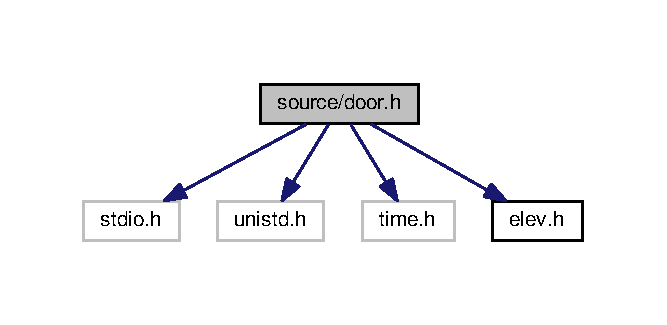
\includegraphics[width=320pt]{door_8h__incl}
\end{center}
\end{figure}
This graph shows which files directly or indirectly include this file\+:\nopagebreak
\begin{figure}[H]
\begin{center}
\leavevmode
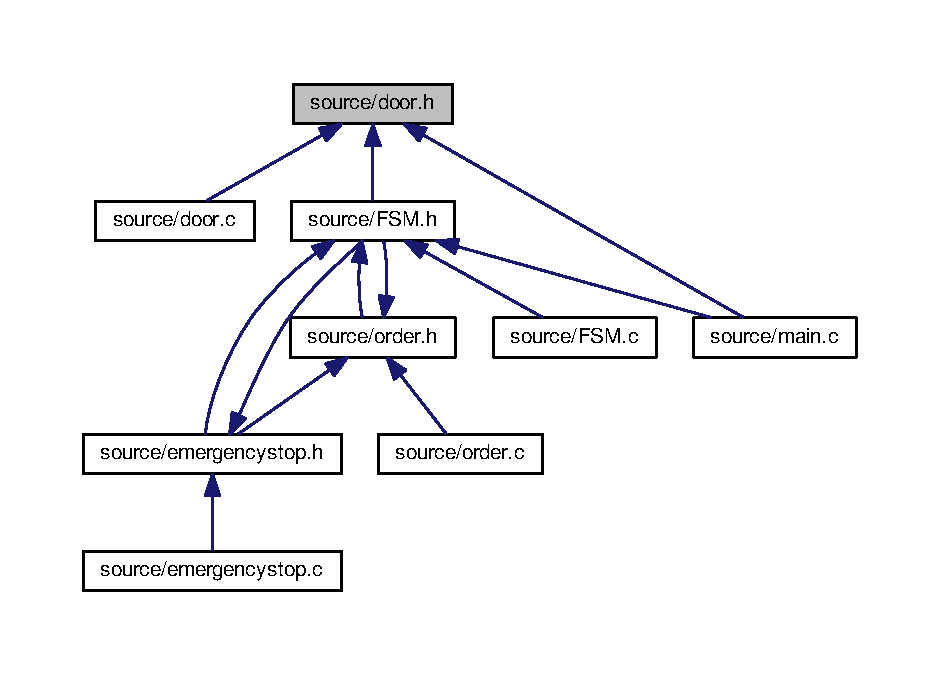
\includegraphics[width=350pt]{door_8h__dep__incl}
\end{center}
\end{figure}
\subsection*{Functions}
\begin{DoxyCompactItemize}
\item 
void \hyperlink{door_8h_a1458972491836d9ac65526b3ca4a6c35}{init\+\_\+door} ()
\item 
int \hyperlink{door_8h_a995f76ec3fd159af2684f7f7a11055e5}{timer\+Done\+\_\+door} ()
\end{DoxyCompactItemize}


\subsection{Detailed Description}
door module, handles door open functionality, ensures the door is opened for 3 seconds then closed again when taking an order. 



\subsection{Function Documentation}
\index{door.\+h@{door.\+h}!init\+\_\+door@{init\+\_\+door}}
\index{init\+\_\+door@{init\+\_\+door}!door.\+h@{door.\+h}}
\subsubsection[{\texorpdfstring{init\+\_\+door()}{init_door()}}]{\setlength{\rightskip}{0pt plus 5cm}void init\+\_\+door (
\begin{DoxyParamCaption}
{}
\end{DoxyParamCaption}
)}\hypertarget{door_8h_a1458972491836d9ac65526b3ca4a6c35}{}\label{door_8h_a1458972491836d9ac65526b3ca4a6c35}
Initializes door state. Stops lift, sets door open light and starts 3sek door open timer. 

Definition at line 3 of file door.\+c.

\index{door.\+h@{door.\+h}!timer\+Done\+\_\+door@{timer\+Done\+\_\+door}}
\index{timer\+Done\+\_\+door@{timer\+Done\+\_\+door}!door.\+h@{door.\+h}}
\subsubsection[{\texorpdfstring{timer\+Done\+\_\+door()}{timerDone_door()}}]{\setlength{\rightskip}{0pt plus 5cm}int timer\+Done\+\_\+door (
\begin{DoxyParamCaption}
{}
\end{DoxyParamCaption}
)}\hypertarget{door_8h_a995f76ec3fd159af2684f7f7a11055e5}{}\label{door_8h_a995f76ec3fd159af2684f7f7a11055e5}
Checks if timer is done for door open state, meaning that 3sek has passed since \hyperlink{door_8h_a1458972491836d9ac65526b3ca4a6c35}{init\+\_\+door()} was called. \begin{DoxyReturn}{Returns}
0 if timer isnt done. 1 if timer is done. 
\end{DoxyReturn}


Definition at line 9 of file door.\+c.


\hypertarget{elev_8h}{}\section{source/elev.h File Reference}
\label{elev_8h}\index{source/elev.\+h@{source/elev.\+h}}


elev module.  


This graph shows which files directly or indirectly include this file\+:\nopagebreak
\begin{figure}[H]
\begin{center}
\leavevmode
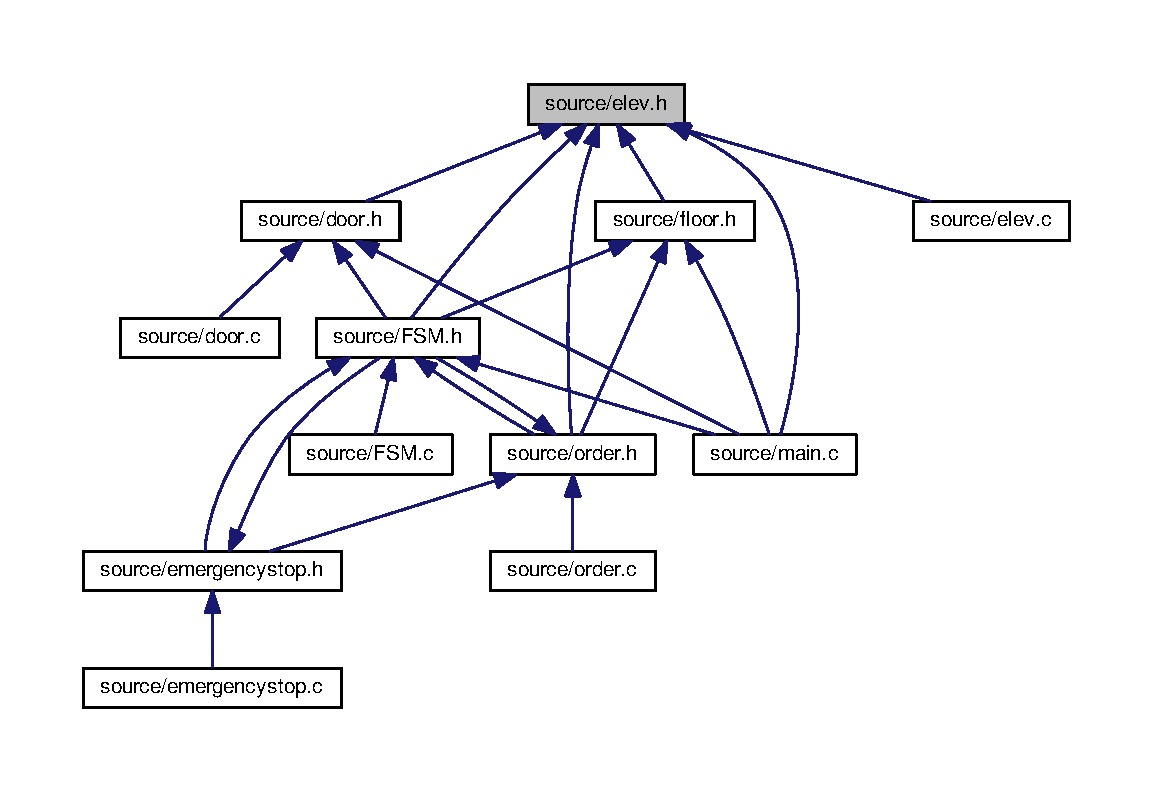
\includegraphics[width=350pt]{elev_8h__dep__incl}
\end{center}
\end{figure}
\subsection*{Macros}
\begin{DoxyCompactItemize}
\item 
\#define {\bfseries N\+\_\+\+F\+L\+O\+O\+RS}~4\hypertarget{elev_8h_ae0592e3739e5e1e76234bb1caf9d1305}{}\label{elev_8h_ae0592e3739e5e1e76234bb1caf9d1305}

\end{DoxyCompactItemize}
\subsection*{Typedefs}
\begin{DoxyCompactItemize}
\item 
typedef enum \hyperlink{elev_8h_aaf85d173ea1bbd3d99c5a2fcf58cba11}{tag\+\_\+elev\+\_\+motor\+\_\+direction} \hyperlink{elev_8h_a2256dfd58fecce253106f83fd2ed607f}{elev\+\_\+motor\+\_\+direction\+\_\+t}
\item 
typedef enum \hyperlink{elev_8h_a0c3f8374e6ebcc71f91341eb3ba6f6f9}{tag\+\_\+elev\+\_\+lamp\+\_\+type} \hyperlink{elev_8h_af61c4136fb437a2c49037e5a57c9abda}{elev\+\_\+button\+\_\+type\+\_\+t}
\end{DoxyCompactItemize}
\subsection*{Enumerations}
\begin{DoxyCompactItemize}
\item 
enum \hyperlink{elev_8h_aaf85d173ea1bbd3d99c5a2fcf58cba11}{tag\+\_\+elev\+\_\+motor\+\_\+direction} \{ {\bfseries D\+I\+R\+N\+\_\+\+D\+O\+WN} = -\/1, 
{\bfseries D\+I\+R\+N\+\_\+\+S\+T\+OP} = 0, 
{\bfseries D\+I\+R\+N\+\_\+\+UP} = 1
 \}
\item 
enum \hyperlink{elev_8h_a0c3f8374e6ebcc71f91341eb3ba6f6f9}{tag\+\_\+elev\+\_\+lamp\+\_\+type} \{ {\bfseries B\+U\+T\+T\+O\+N\+\_\+\+C\+A\+L\+L\+\_\+\+UP} = 0, 
{\bfseries B\+U\+T\+T\+O\+N\+\_\+\+C\+A\+L\+L\+\_\+\+D\+O\+WN} = 1, 
{\bfseries B\+U\+T\+T\+O\+N\+\_\+\+C\+O\+M\+M\+A\+ND} = 2
 \}
\end{DoxyCompactItemize}
\subsection*{Functions}
\begin{DoxyCompactItemize}
\item 
int \hyperlink{elev_8h_a949b0e1f7c0f03ea6f92008c378e4573}{elev\+\_\+init} (void)
\item 
void \hyperlink{elev_8h_ac7dccb879f6e812e9d245174a0214536}{elev\+\_\+set\+\_\+motor\+\_\+direction} (\hyperlink{elev_8h_a2256dfd58fecce253106f83fd2ed607f}{elev\+\_\+motor\+\_\+direction\+\_\+t} dirn)
\item 
void \hyperlink{elev_8h_a6ce9a34b8677b483b0d8f9dc47b42c40}{elev\+\_\+set\+\_\+door\+\_\+open\+\_\+lamp} (int value)
\item 
int \hyperlink{elev_8h_acd97a0fbc9013dc954923e25e90be9df}{elev\+\_\+get\+\_\+obstruction\+\_\+signal} (void)
\item 
int \hyperlink{elev_8h_ab702d0ff2d7d03172b7ae3829ba13028}{elev\+\_\+get\+\_\+stop\+\_\+signal} (void)
\item 
void \hyperlink{elev_8h_a85de2a6536b4dd0c83bac19923500740}{elev\+\_\+set\+\_\+stop\+\_\+lamp} (int value)
\item 
int \hyperlink{elev_8h_a97d30b7e2538acf5647515638070fdc5}{elev\+\_\+get\+\_\+floor\+\_\+sensor\+\_\+signal} (void)
\item 
void \hyperlink{elev_8h_a6af53dd3ebae3a5791ba345eac84d4be}{elev\+\_\+set\+\_\+floor\+\_\+indicator} (int floor)
\item 
int \hyperlink{elev_8h_a2350a1635233760719700552a6cb0763}{elev\+\_\+get\+\_\+button\+\_\+signal} (\hyperlink{elev_8h_af61c4136fb437a2c49037e5a57c9abda}{elev\+\_\+button\+\_\+type\+\_\+t} button, int floor)
\item 
void \hyperlink{elev_8h_a9e81321c63d80ddf1699bc91593cd9d4}{elev\+\_\+set\+\_\+button\+\_\+lamp} (\hyperlink{elev_8h_af61c4136fb437a2c49037e5a57c9abda}{elev\+\_\+button\+\_\+type\+\_\+t} button, int floor, int value)
\end{DoxyCompactItemize}


\subsection{Detailed Description}
elev module. 



\subsection{Typedef Documentation}
\index{elev.\+h@{elev.\+h}!elev\+\_\+button\+\_\+type\+\_\+t@{elev\+\_\+button\+\_\+type\+\_\+t}}
\index{elev\+\_\+button\+\_\+type\+\_\+t@{elev\+\_\+button\+\_\+type\+\_\+t}!elev.\+h@{elev.\+h}}
\subsubsection[{\texorpdfstring{elev\+\_\+button\+\_\+type\+\_\+t}{elev_button_type_t}}]{\setlength{\rightskip}{0pt plus 5cm}typedef enum {\bf tag\+\_\+elev\+\_\+lamp\+\_\+type}  {\bf elev\+\_\+button\+\_\+type\+\_\+t}}\hypertarget{elev_8h_af61c4136fb437a2c49037e5a57c9abda}{}\label{elev_8h_af61c4136fb437a2c49037e5a57c9abda}
Button types for function \hyperlink{elev_8h_a9e81321c63d80ddf1699bc91593cd9d4}{elev\+\_\+set\+\_\+button\+\_\+lamp()} and elev\+\_\+get\+\_\+button(). \index{elev.\+h@{elev.\+h}!elev\+\_\+motor\+\_\+direction\+\_\+t@{elev\+\_\+motor\+\_\+direction\+\_\+t}}
\index{elev\+\_\+motor\+\_\+direction\+\_\+t@{elev\+\_\+motor\+\_\+direction\+\_\+t}!elev.\+h@{elev.\+h}}
\subsubsection[{\texorpdfstring{elev\+\_\+motor\+\_\+direction\+\_\+t}{elev_motor_direction_t}}]{\setlength{\rightskip}{0pt plus 5cm}typedef enum {\bf tag\+\_\+elev\+\_\+motor\+\_\+direction}  {\bf elev\+\_\+motor\+\_\+direction\+\_\+t}}\hypertarget{elev_8h_a2256dfd58fecce253106f83fd2ed607f}{}\label{elev_8h_a2256dfd58fecce253106f83fd2ed607f}
Motor direction for function \hyperlink{elev_8h_ac7dccb879f6e812e9d245174a0214536}{elev\+\_\+set\+\_\+motor\+\_\+direction()}. 

\subsection{Enumeration Type Documentation}
\index{elev.\+h@{elev.\+h}!tag\+\_\+elev\+\_\+lamp\+\_\+type@{tag\+\_\+elev\+\_\+lamp\+\_\+type}}
\index{tag\+\_\+elev\+\_\+lamp\+\_\+type@{tag\+\_\+elev\+\_\+lamp\+\_\+type}!elev.\+h@{elev.\+h}}
\subsubsection[{\texorpdfstring{tag\+\_\+elev\+\_\+lamp\+\_\+type}{tag_elev_lamp_type}}]{\setlength{\rightskip}{0pt plus 5cm}enum {\bf tag\+\_\+elev\+\_\+lamp\+\_\+type}}\hypertarget{elev_8h_a0c3f8374e6ebcc71f91341eb3ba6f6f9}{}\label{elev_8h_a0c3f8374e6ebcc71f91341eb3ba6f6f9}
Button types for function \hyperlink{elev_8h_a9e81321c63d80ddf1699bc91593cd9d4}{elev\+\_\+set\+\_\+button\+\_\+lamp()} and elev\+\_\+get\+\_\+button(). 

Definition at line 97 of file elev.\+h.

\index{elev.\+h@{elev.\+h}!tag\+\_\+elev\+\_\+motor\+\_\+direction@{tag\+\_\+elev\+\_\+motor\+\_\+direction}}
\index{tag\+\_\+elev\+\_\+motor\+\_\+direction@{tag\+\_\+elev\+\_\+motor\+\_\+direction}!elev.\+h@{elev.\+h}}
\subsubsection[{\texorpdfstring{tag\+\_\+elev\+\_\+motor\+\_\+direction}{tag_elev_motor_direction}}]{\setlength{\rightskip}{0pt plus 5cm}enum {\bf tag\+\_\+elev\+\_\+motor\+\_\+direction}}\hypertarget{elev_8h_aaf85d173ea1bbd3d99c5a2fcf58cba11}{}\label{elev_8h_aaf85d173ea1bbd3d99c5a2fcf58cba11}
Motor direction for function \hyperlink{elev_8h_ac7dccb879f6e812e9d245174a0214536}{elev\+\_\+set\+\_\+motor\+\_\+direction()}. 

Definition at line 29 of file elev.\+h.



\subsection{Function Documentation}
\index{elev.\+h@{elev.\+h}!elev\+\_\+get\+\_\+button\+\_\+signal@{elev\+\_\+get\+\_\+button\+\_\+signal}}
\index{elev\+\_\+get\+\_\+button\+\_\+signal@{elev\+\_\+get\+\_\+button\+\_\+signal}!elev.\+h@{elev.\+h}}
\subsubsection[{\texorpdfstring{elev\+\_\+get\+\_\+button\+\_\+signal(elev\+\_\+button\+\_\+type\+\_\+t button, int floor)}{elev_get_button_signal(elev_button_type_t button, int floor)}}]{\setlength{\rightskip}{0pt plus 5cm}int elev\+\_\+get\+\_\+button\+\_\+signal (
\begin{DoxyParamCaption}
\item[{{\bf elev\+\_\+button\+\_\+type\+\_\+t}}]{button, }
\item[{int}]{floor}
\end{DoxyParamCaption}
)}\hypertarget{elev_8h_a2350a1635233760719700552a6cb0763}{}\label{elev_8h_a2350a1635233760719700552a6cb0763}
Gets a button signal. 
\begin{DoxyParams}{Parameters}
{\em button} & Which button type to check. Can be B\+U\+T\+T\+O\+N\+\_\+\+C\+A\+L\+L\+\_\+\+UP, B\+U\+T\+T\+O\+N\+\_\+\+C\+A\+L\+L\+\_\+\+D\+O\+WN or B\+U\+T\+T\+O\+N\+\_\+\+C\+O\+M\+M\+A\+ND (button "inside the elevator). \\
\hline
{\em floor} & Which floor to check button. Must be 0-\/3. \\
\hline
\end{DoxyParams}
\begin{DoxyReturn}{Returns}
0 if button is not pushed. 1 if button is pushed. 
\end{DoxyReturn}


Definition at line 122 of file elev.\+c.

\index{elev.\+h@{elev.\+h}!elev\+\_\+get\+\_\+floor\+\_\+sensor\+\_\+signal@{elev\+\_\+get\+\_\+floor\+\_\+sensor\+\_\+signal}}
\index{elev\+\_\+get\+\_\+floor\+\_\+sensor\+\_\+signal@{elev\+\_\+get\+\_\+floor\+\_\+sensor\+\_\+signal}!elev.\+h@{elev.\+h}}
\subsubsection[{\texorpdfstring{elev\+\_\+get\+\_\+floor\+\_\+sensor\+\_\+signal(void)}{elev_get_floor_sensor_signal(void)}}]{\setlength{\rightskip}{0pt plus 5cm}int elev\+\_\+get\+\_\+floor\+\_\+sensor\+\_\+signal (
\begin{DoxyParamCaption}
\item[{void}]{}
\end{DoxyParamCaption}
)}\hypertarget{elev_8h_a97d30b7e2538acf5647515638070fdc5}{}\label{elev_8h_a97d30b7e2538acf5647515638070fdc5}
Get floor sensor signal. \begin{DoxyReturn}{Returns}
-\/1 if elevator is not on a floor. 0-\/3 if elevator is on floor. 0 is ground floor, 3 is top floor. 
\end{DoxyReturn}


Definition at line 93 of file elev.\+c.

\index{elev.\+h@{elev.\+h}!elev\+\_\+get\+\_\+obstruction\+\_\+signal@{elev\+\_\+get\+\_\+obstruction\+\_\+signal}}
\index{elev\+\_\+get\+\_\+obstruction\+\_\+signal@{elev\+\_\+get\+\_\+obstruction\+\_\+signal}!elev.\+h@{elev.\+h}}
\subsubsection[{\texorpdfstring{elev\+\_\+get\+\_\+obstruction\+\_\+signal(void)}{elev_get_obstruction_signal(void)}}]{\setlength{\rightskip}{0pt plus 5cm}int elev\+\_\+get\+\_\+obstruction\+\_\+signal (
\begin{DoxyParamCaption}
\item[{void}]{}
\end{DoxyParamCaption}
)}\hypertarget{elev_8h_acd97a0fbc9013dc954923e25e90be9df}{}\label{elev_8h_acd97a0fbc9013dc954923e25e90be9df}
Get signal from obstruction switch. \begin{DoxyReturn}{Returns}
1 if obstruction is enabled. 0 if not. 
\end{DoxyReturn}


Definition at line 78 of file elev.\+c.

\index{elev.\+h@{elev.\+h}!elev\+\_\+get\+\_\+stop\+\_\+signal@{elev\+\_\+get\+\_\+stop\+\_\+signal}}
\index{elev\+\_\+get\+\_\+stop\+\_\+signal@{elev\+\_\+get\+\_\+stop\+\_\+signal}!elev.\+h@{elev.\+h}}
\subsubsection[{\texorpdfstring{elev\+\_\+get\+\_\+stop\+\_\+signal(void)}{elev_get_stop_signal(void)}}]{\setlength{\rightskip}{0pt plus 5cm}int elev\+\_\+get\+\_\+stop\+\_\+signal (
\begin{DoxyParamCaption}
\item[{void}]{}
\end{DoxyParamCaption}
)}\hypertarget{elev_8h_ab702d0ff2d7d03172b7ae3829ba13028}{}\label{elev_8h_ab702d0ff2d7d03172b7ae3829ba13028}
Get signal from stop button. \begin{DoxyReturn}{Returns}
1 if stop button is pushed, 0 if not. 
\end{DoxyReturn}


Definition at line 82 of file elev.\+c.

\index{elev.\+h@{elev.\+h}!elev\+\_\+init@{elev\+\_\+init}}
\index{elev\+\_\+init@{elev\+\_\+init}!elev.\+h@{elev.\+h}}
\subsubsection[{\texorpdfstring{elev\+\_\+init(void)}{elev_init(void)}}]{\setlength{\rightskip}{0pt plus 5cm}int elev\+\_\+init (
\begin{DoxyParamCaption}
\item[{void}]{}
\end{DoxyParamCaption}
)}\hypertarget{elev_8h_a949b0e1f7c0f03ea6f92008c378e4573}{}\label{elev_8h_a949b0e1f7c0f03ea6f92008c378e4573}
Initialize elevator. \begin{DoxyReturn}{Returns}
Non-\/zero on success, 0 on failure. 
\end{DoxyReturn}


Definition at line 32 of file elev.\+c.

\index{elev.\+h@{elev.\+h}!elev\+\_\+set\+\_\+button\+\_\+lamp@{elev\+\_\+set\+\_\+button\+\_\+lamp}}
\index{elev\+\_\+set\+\_\+button\+\_\+lamp@{elev\+\_\+set\+\_\+button\+\_\+lamp}!elev.\+h@{elev.\+h}}
\subsubsection[{\texorpdfstring{elev\+\_\+set\+\_\+button\+\_\+lamp(elev\+\_\+button\+\_\+type\+\_\+t button, int floor, int value)}{elev_set_button_lamp(elev_button_type_t button, int floor, int value)}}]{\setlength{\rightskip}{0pt plus 5cm}void elev\+\_\+set\+\_\+button\+\_\+lamp (
\begin{DoxyParamCaption}
\item[{{\bf elev\+\_\+button\+\_\+type\+\_\+t}}]{button, }
\item[{int}]{floor, }
\item[{int}]{value}
\end{DoxyParamCaption}
)}\hypertarget{elev_8h_a9e81321c63d80ddf1699bc91593cd9d4}{}\label{elev_8h_a9e81321c63d80ddf1699bc91593cd9d4}
Set a button lamp. 
\begin{DoxyParams}{Parameters}
{\em lamp} & Which type of lamp to set. Can be B\+U\+T\+T\+O\+N\+\_\+\+C\+A\+L\+L\+\_\+\+UP, B\+U\+T\+T\+O\+N\+\_\+\+C\+A\+L\+L\+\_\+\+D\+O\+WN or B\+U\+T\+T\+O\+N\+\_\+\+C\+O\+M\+M\+A\+ND (button \char`\"{}inside\char`\"{} the elevator). \\
\hline
{\em floor} & Floor of lamp to set. Must be 0-\/3 \\
\hline
{\em value} & Non-\/zero value turns lamp on, 0 turns lamp off. \\
\hline
\end{DoxyParams}


Definition at line 135 of file elev.\+c.

\index{elev.\+h@{elev.\+h}!elev\+\_\+set\+\_\+door\+\_\+open\+\_\+lamp@{elev\+\_\+set\+\_\+door\+\_\+open\+\_\+lamp}}
\index{elev\+\_\+set\+\_\+door\+\_\+open\+\_\+lamp@{elev\+\_\+set\+\_\+door\+\_\+open\+\_\+lamp}!elev.\+h@{elev.\+h}}
\subsubsection[{\texorpdfstring{elev\+\_\+set\+\_\+door\+\_\+open\+\_\+lamp(int value)}{elev_set_door_open_lamp(int value)}}]{\setlength{\rightskip}{0pt plus 5cm}void elev\+\_\+set\+\_\+door\+\_\+open\+\_\+lamp (
\begin{DoxyParamCaption}
\item[{int}]{value}
\end{DoxyParamCaption}
)}\hypertarget{elev_8h_a6ce9a34b8677b483b0d8f9dc47b42c40}{}\label{elev_8h_a6ce9a34b8677b483b0d8f9dc47b42c40}
Turn door-\/open lamp on or off. 
\begin{DoxyParams}{Parameters}
{\em value} & Non-\/zero value turns lamp on, 0 turns lamp off. \\
\hline
\end{DoxyParams}


Definition at line 71 of file elev.\+c.

\index{elev.\+h@{elev.\+h}!elev\+\_\+set\+\_\+floor\+\_\+indicator@{elev\+\_\+set\+\_\+floor\+\_\+indicator}}
\index{elev\+\_\+set\+\_\+floor\+\_\+indicator@{elev\+\_\+set\+\_\+floor\+\_\+indicator}!elev.\+h@{elev.\+h}}
\subsubsection[{\texorpdfstring{elev\+\_\+set\+\_\+floor\+\_\+indicator(int floor)}{elev_set_floor_indicator(int floor)}}]{\setlength{\rightskip}{0pt plus 5cm}void elev\+\_\+set\+\_\+floor\+\_\+indicator (
\begin{DoxyParamCaption}
\item[{int}]{floor}
\end{DoxyParamCaption}
)}\hypertarget{elev_8h_a6af53dd3ebae3a5791ba345eac84d4be}{}\label{elev_8h_a6af53dd3ebae3a5791ba345eac84d4be}
Set floor indicator lamp for a given floor. 
\begin{DoxyParams}{Parameters}
{\em floor} & Which floor lamp to turn on. Other floor lamps are turned off. \\
\hline
\end{DoxyParams}


Definition at line 106 of file elev.\+c.

\index{elev.\+h@{elev.\+h}!elev\+\_\+set\+\_\+motor\+\_\+direction@{elev\+\_\+set\+\_\+motor\+\_\+direction}}
\index{elev\+\_\+set\+\_\+motor\+\_\+direction@{elev\+\_\+set\+\_\+motor\+\_\+direction}!elev.\+h@{elev.\+h}}
\subsubsection[{\texorpdfstring{elev\+\_\+set\+\_\+motor\+\_\+direction(elev\+\_\+motor\+\_\+direction\+\_\+t dirn)}{elev_set_motor_direction(elev_motor_direction_t dirn)}}]{\setlength{\rightskip}{0pt plus 5cm}void elev\+\_\+set\+\_\+motor\+\_\+direction (
\begin{DoxyParamCaption}
\item[{{\bf elev\+\_\+motor\+\_\+direction\+\_\+t}}]{dirn}
\end{DoxyParamCaption}
)}\hypertarget{elev_8h_ac7dccb879f6e812e9d245174a0214536}{}\label{elev_8h_ac7dccb879f6e812e9d245174a0214536}
Sets the motor direction of the elevator. 
\begin{DoxyParams}{Parameters}
{\em dirn} & New direction of the elevator. \\
\hline
\end{DoxyParams}


Definition at line 59 of file elev.\+c.

\index{elev.\+h@{elev.\+h}!elev\+\_\+set\+\_\+stop\+\_\+lamp@{elev\+\_\+set\+\_\+stop\+\_\+lamp}}
\index{elev\+\_\+set\+\_\+stop\+\_\+lamp@{elev\+\_\+set\+\_\+stop\+\_\+lamp}!elev.\+h@{elev.\+h}}
\subsubsection[{\texorpdfstring{elev\+\_\+set\+\_\+stop\+\_\+lamp(int value)}{elev_set_stop_lamp(int value)}}]{\setlength{\rightskip}{0pt plus 5cm}void elev\+\_\+set\+\_\+stop\+\_\+lamp (
\begin{DoxyParamCaption}
\item[{int}]{value}
\end{DoxyParamCaption}
)}\hypertarget{elev_8h_a85de2a6536b4dd0c83bac19923500740}{}\label{elev_8h_a85de2a6536b4dd0c83bac19923500740}
Turn stop lamp on or off. 
\begin{DoxyParams}{Parameters}
{\em value} & Non-\/zero value turns lamp on, 0 turns lamp off. \\
\hline
\end{DoxyParams}


Definition at line 86 of file elev.\+c.


\hypertarget{emergencystop_8h}{}\section{source/emergencystop.h File Reference}
\label{emergencystop_8h}\index{source/emergencystop.\+h@{source/emergencystop.\+h}}


emergency stop module, makes sure lift stops immediately and all orders removed when the stop button is pressed.  


{\ttfamily \#include \char`\"{}F\+S\+M.\+h\char`\"{}}\\*
{\ttfamily \#include \char`\"{}order.\+h\char`\"{}}\\*
Include dependency graph for emergencystop.\+h\+:\nopagebreak
\begin{figure}[H]
\begin{center}
\leavevmode
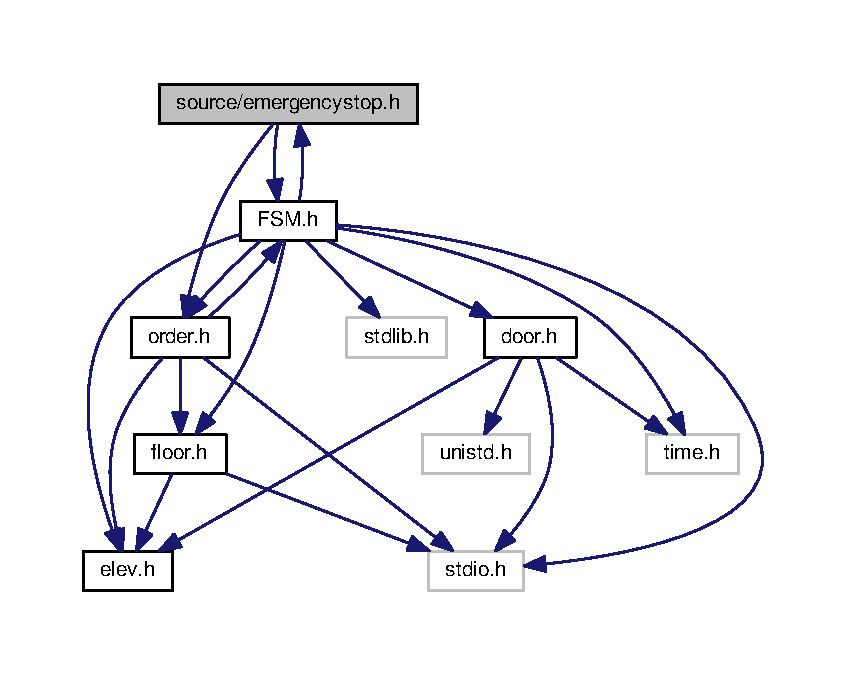
\includegraphics[width=350pt]{emergencystop_8h__incl}
\end{center}
\end{figure}
This graph shows which files directly or indirectly include this file\+:\nopagebreak
\begin{figure}[H]
\begin{center}
\leavevmode
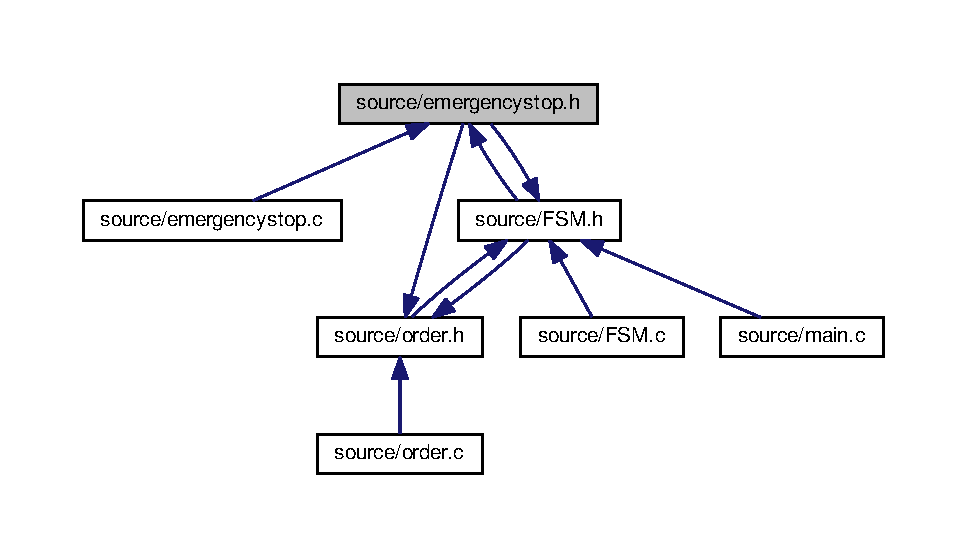
\includegraphics[width=350pt]{emergencystop_8h__dep__incl}
\end{center}
\end{figure}
\subsection*{Functions}
\begin{DoxyCompactItemize}
\item 
void \hyperlink{emergencystop_8h_a1c601ddde02b05975511908acb494756}{init\+\_\+emergencystop} ()
\end{DoxyCompactItemize}


\subsection{Detailed Description}
emergency stop module, makes sure lift stops immediately and all orders removed when the stop button is pressed. 



\subsection{Function Documentation}
\index{emergencystop.\+h@{emergencystop.\+h}!init\+\_\+emergencystop@{init\+\_\+emergencystop}}
\index{init\+\_\+emergencystop@{init\+\_\+emergencystop}!emergencystop.\+h@{emergencystop.\+h}}
\subsubsection[{\texorpdfstring{init\+\_\+emergencystop()}{init_emergencystop()}}]{\setlength{\rightskip}{0pt plus 5cm}void init\+\_\+emergencystop (
\begin{DoxyParamCaption}
{}
\end{DoxyParamCaption}
)}\hypertarget{emergencystop_8h_a1c601ddde02b05975511908acb494756}{}\label{emergencystop_8h_a1c601ddde02b05975511908acb494756}
Initializes emergency stop state. immediately stops lift, sets stop lamp, removes all orders. 

Definition at line 3 of file emergencystop.\+c.


\hypertarget{floor_8h}{}\section{source/floor.h File Reference}
\label{floor_8h}\index{source/floor.\+h@{source/floor.\+h}}


floor module, containing the floor enum.  


{\ttfamily \#include \char`\"{}elev.\+h\char`\"{}}\\*
{\ttfamily \#include $<$stdio.\+h$>$}\\*
Include dependency graph for floor.\+h\+:\nopagebreak
\begin{figure}[H]
\begin{center}
\leavevmode
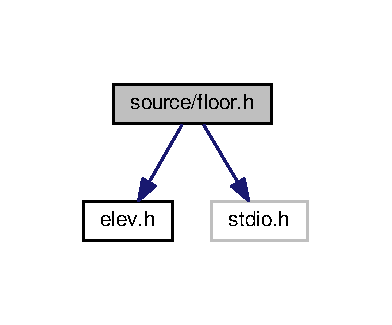
\includegraphics[width=188pt]{floor_8h__incl}
\end{center}
\end{figure}
This graph shows which files directly or indirectly include this file\+:\nopagebreak
\begin{figure}[H]
\begin{center}
\leavevmode
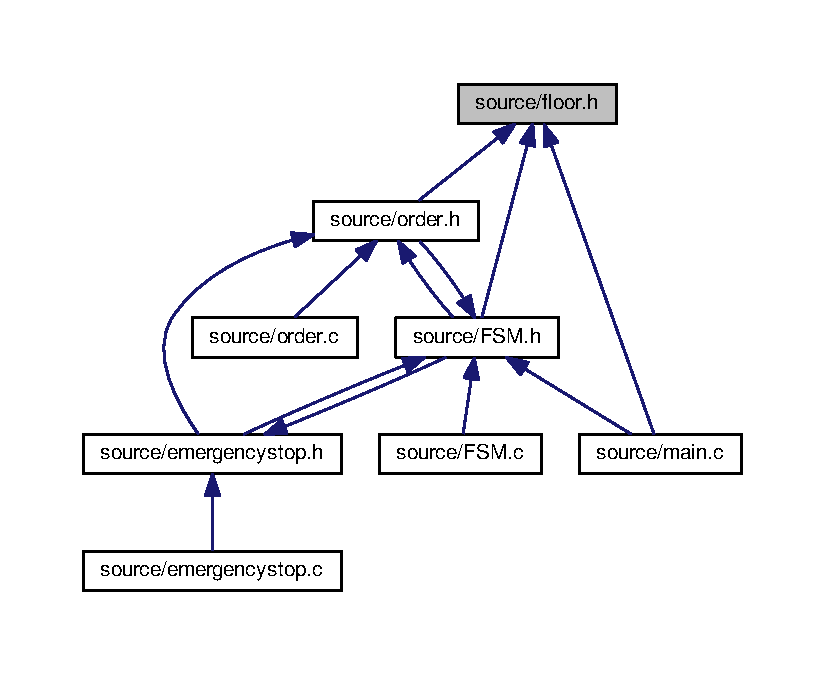
\includegraphics[width=350pt]{floor_8h__dep__incl}
\end{center}
\end{figure}
\subsection*{Typedefs}
\begin{DoxyCompactItemize}
\item 
typedef enum \hyperlink{floor_8h_a31c3d890453e9b6491fbb0a0a6bab5f9}{tag\+\_\+floor} \hyperlink{floor_8h_acb30631293fda569568eff832f5185b4}{Floor}
\end{DoxyCompactItemize}
\subsection*{Enumerations}
\begin{DoxyCompactItemize}
\item 
enum \hyperlink{floor_8h_a31c3d890453e9b6491fbb0a0a6bab5f9}{tag\+\_\+floor} \{ \\*
{\bfseries U\+N\+D\+E\+F\+I\+N\+ED} = -\/1, 
{\bfseries F\+I\+R\+ST} = 0, 
{\bfseries S\+E\+C\+O\+ND} = 1, 
{\bfseries T\+H\+I\+RD} = 2, 
\\*
{\bfseries F\+O\+U\+R\+TH} = 3
 \}
\end{DoxyCompactItemize}


\subsection{Detailed Description}
floor module, containing the floor enum. 



\subsection{Typedef Documentation}
\index{floor.\+h@{floor.\+h}!Floor@{Floor}}
\index{Floor@{Floor}!floor.\+h@{floor.\+h}}
\subsubsection[{\texorpdfstring{Floor}{Floor}}]{\setlength{\rightskip}{0pt plus 5cm}typedef enum {\bf tag\+\_\+floor}  {\bf Floor}}\hypertarget{floor_8h_acb30631293fda569568eff832f5185b4}{}\label{floor_8h_acb30631293fda569568eff832f5185b4}
Enum with the discrete floors of the lift, {\ttfamily U\+N\+D\+E\+F\+I\+N\+ED}, {\ttfamily F\+I\+R\+ST}, {\ttfamily S\+E\+C\+O\+ND}, {\ttfamily T\+H\+I\+RD}, {\ttfamily F\+O\+U\+R\+TH} 

\subsection{Enumeration Type Documentation}
\index{floor.\+h@{floor.\+h}!tag\+\_\+floor@{tag\+\_\+floor}}
\index{tag\+\_\+floor@{tag\+\_\+floor}!floor.\+h@{floor.\+h}}
\subsubsection[{\texorpdfstring{tag\+\_\+floor}{tag_floor}}]{\setlength{\rightskip}{0pt plus 5cm}enum {\bf tag\+\_\+floor}}\hypertarget{floor_8h_a31c3d890453e9b6491fbb0a0a6bab5f9}{}\label{floor_8h_a31c3d890453e9b6491fbb0a0a6bab5f9}
Enum with the discrete floors of the lift, {\ttfamily U\+N\+D\+E\+F\+I\+N\+ED}, {\ttfamily F\+I\+R\+ST}, {\ttfamily S\+E\+C\+O\+ND}, {\ttfamily T\+H\+I\+RD}, {\ttfamily F\+O\+U\+R\+TH} 

Definition at line 16 of file floor.\+h.


\hypertarget{FSM_8h}{}\section{source/\+F\+SM.h File Reference}
\label{FSM_8h}\index{source/\+F\+S\+M.\+h@{source/\+F\+S\+M.\+h}}


Finite state machine, switches between the 4 finite states {\ttfamily I\+D\+LE}, {\ttfamily R\+U\+N\+N\+I\+NG}, {\ttfamily D\+O\+O\+R\+\_\+\+O\+P\+EN}, {\ttfamily E\+M\+E\+R\+G\+E\+N\+C\+Y\+S\+T\+OP}.  


{\ttfamily \#include \char`\"{}door.\+h\char`\"{}}\\*
{\ttfamily \#include \char`\"{}elev.\+h\char`\"{}}\\*
{\ttfamily \#include \char`\"{}order.\+h\char`\"{}}\\*
{\ttfamily \#include \char`\"{}emergencystop.\+h\char`\"{}}\\*
{\ttfamily \#include \char`\"{}floor.\+h\char`\"{}}\\*
{\ttfamily \#include $<$stdlib.\+h$>$}\\*
{\ttfamily \#include $<$stdio.\+h$>$}\\*
{\ttfamily \#include $<$time.\+h$>$}\\*
Include dependency graph for F\+S\+M.\+h\+:\nopagebreak
\begin{figure}[H]
\begin{center}
\leavevmode
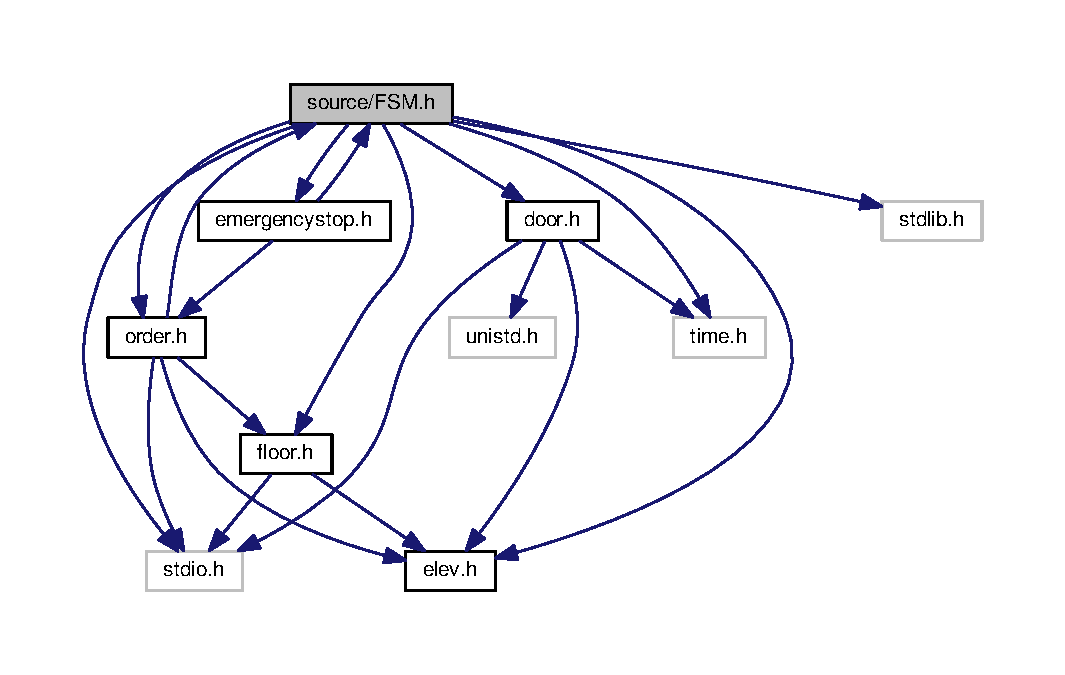
\includegraphics[width=350pt]{FSM_8h__incl}
\end{center}
\end{figure}
This graph shows which files directly or indirectly include this file\+:\nopagebreak
\begin{figure}[H]
\begin{center}
\leavevmode
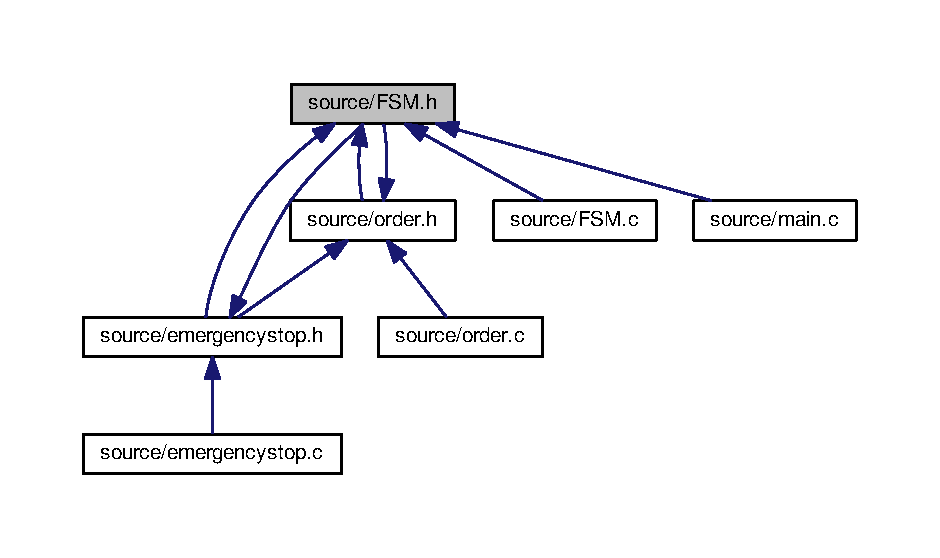
\includegraphics[width=350pt]{FSM_8h__dep__incl}
\end{center}
\end{figure}
\subsection*{Typedefs}
\begin{DoxyCompactItemize}
\item 
typedef enum \hyperlink{FSM_8h_a2af5bc6b2437cab9b3dd701744368abf}{tag\+\_\+state} \hyperlink{FSM_8h_ad278733225752463f5d2037c57b641d0}{State}
\end{DoxyCompactItemize}
\subsection*{Enumerations}
\begin{DoxyCompactItemize}
\item 
enum \hyperlink{FSM_8h_a2af5bc6b2437cab9b3dd701744368abf}{tag\+\_\+state} \{ {\bfseries I\+D\+LE} = 1, 
{\bfseries R\+U\+N\+N\+I\+NG}, 
{\bfseries D\+O\+O\+R\+\_\+\+O\+P\+EN}, 
{\bfseries E\+M\+E\+R\+G\+E\+N\+C\+Y\+S\+T\+OP}
 \}
\end{DoxyCompactItemize}
\subsection*{Functions}
\begin{DoxyCompactItemize}
\item 
void \hyperlink{FSM_8h_a005388f6e2fad37bb0824bf92193c865}{init\+\_\+\+F\+SM} ()
\item 
void \hyperlink{FSM_8h_a891efeca975caaa8422495176292f2aa}{F\+SM} ()
\item 
void \hyperlink{FSM_8h_ab35866a9fcf9da539677d0c3e910a245}{Print\+State\+\_\+\+F\+SM} (\hyperlink{FSM_8h_ad278733225752463f5d2037c57b641d0}{State} state)
\end{DoxyCompactItemize}


\subsection{Detailed Description}
Finite state machine, switches between the 4 finite states {\ttfamily I\+D\+LE}, {\ttfamily R\+U\+N\+N\+I\+NG}, {\ttfamily D\+O\+O\+R\+\_\+\+O\+P\+EN}, {\ttfamily E\+M\+E\+R\+G\+E\+N\+C\+Y\+S\+T\+OP}. 



\subsection{Typedef Documentation}
\index{F\+S\+M.\+h@{F\+S\+M.\+h}!State@{State}}
\index{State@{State}!F\+S\+M.\+h@{F\+S\+M.\+h}}
\subsubsection[{\texorpdfstring{State}{State}}]{\setlength{\rightskip}{0pt plus 5cm}typedef enum {\bf tag\+\_\+state}  {\bf State}}\hypertarget{FSM_8h_ad278733225752463f5d2037c57b641d0}{}\label{FSM_8h_ad278733225752463f5d2037c57b641d0}
The states the finite state machine can be in, {\ttfamily I\+D\+LE}, {\ttfamily R\+U\+N\+N\+I\+NG}, {\ttfamily D\+O\+O\+R\+\_\+\+O\+P\+EN}, {\ttfamily E\+M\+E\+R\+G\+E\+N\+C\+Y\+S\+T\+OP} 

\subsection{Enumeration Type Documentation}
\index{F\+S\+M.\+h@{F\+S\+M.\+h}!tag\+\_\+state@{tag\+\_\+state}}
\index{tag\+\_\+state@{tag\+\_\+state}!F\+S\+M.\+h@{F\+S\+M.\+h}}
\subsubsection[{\texorpdfstring{tag\+\_\+state}{tag_state}}]{\setlength{\rightskip}{0pt plus 5cm}enum {\bf tag\+\_\+state}}\hypertarget{FSM_8h_a2af5bc6b2437cab9b3dd701744368abf}{}\label{FSM_8h_a2af5bc6b2437cab9b3dd701744368abf}
The states the finite state machine can be in, {\ttfamily I\+D\+LE}, {\ttfamily R\+U\+N\+N\+I\+NG}, {\ttfamily D\+O\+O\+R\+\_\+\+O\+P\+EN}, {\ttfamily E\+M\+E\+R\+G\+E\+N\+C\+Y\+S\+T\+OP} 

Definition at line 28 of file F\+S\+M.\+h.



\subsection{Function Documentation}
\index{F\+S\+M.\+h@{F\+S\+M.\+h}!F\+SM@{F\+SM}}
\index{F\+SM@{F\+SM}!F\+S\+M.\+h@{F\+S\+M.\+h}}
\subsubsection[{\texorpdfstring{F\+S\+M()}{FSM()}}]{\setlength{\rightskip}{0pt plus 5cm}void F\+SM (
\begin{DoxyParamCaption}
{}
\end{DoxyParamCaption}
)}\hypertarget{FSM_8h_a891efeca975caaa8422495176292f2aa}{}\label{FSM_8h_a891efeca975caaa8422495176292f2aa}
Runs the finite state machine. There are 4 states, {\ttfamily E\+M\+E\+R\+G\+E\+N\+C\+Y\+S\+T\+OP}, {\ttfamily D\+O\+O\+R\+\_\+\+O\+P\+EN}, {\ttfamily R\+U\+N\+N\+I\+NG} and {\ttfamily I\+D\+LE} given by struct State. Emergency stop state and door open state are described by their corresponding modules. Running state is moving the lift in the direction given by the order module. In idle the lift is waiting for orders with the doors closed. The transitions between states is shown and explained in the state diagram. 

Definition at line 38 of file F\+S\+M.\+c.

\index{F\+S\+M.\+h@{F\+S\+M.\+h}!init\+\_\+\+F\+SM@{init\+\_\+\+F\+SM}}
\index{init\+\_\+\+F\+SM@{init\+\_\+\+F\+SM}!F\+S\+M.\+h@{F\+S\+M.\+h}}
\subsubsection[{\texorpdfstring{init\+\_\+\+F\+S\+M()}{init_FSM()}}]{\setlength{\rightskip}{0pt plus 5cm}void init\+\_\+\+F\+SM (
\begin{DoxyParamCaption}
{}
\end{DoxyParamCaption}
)}\hypertarget{FSM_8h_a005388f6e2fad37bb0824bf92193c865}{}\label{FSM_8h_a005388f6e2fad37bb0824bf92193c865}
Initializes state machine Initializes lift positition, when position is initialized lift transitions to idle state. 

Definition at line 23 of file F\+S\+M.\+c.

\index{F\+S\+M.\+h@{F\+S\+M.\+h}!Print\+State\+\_\+\+F\+SM@{Print\+State\+\_\+\+F\+SM}}
\index{Print\+State\+\_\+\+F\+SM@{Print\+State\+\_\+\+F\+SM}!F\+S\+M.\+h@{F\+S\+M.\+h}}
\subsubsection[{\texorpdfstring{Print\+State\+\_\+\+F\+S\+M(\+State state)}{PrintState_FSM(State state)}}]{\setlength{\rightskip}{0pt plus 5cm}void Print\+State\+\_\+\+F\+SM (
\begin{DoxyParamCaption}
\item[{{\bf State}}]{state}
\end{DoxyParamCaption}
)}\hypertarget{FSM_8h_ab35866a9fcf9da539677d0c3e910a245}{}\label{FSM_8h_ab35866a9fcf9da539677d0c3e910a245}
Prints state 
\begin{DoxyParams}{Parameters}
{\em state} & Which state to print \\
\hline
\end{DoxyParams}


Definition at line 4 of file F\+S\+M.\+c.


\hypertarget{io_8h}{}\section{source/io.h File Reference}
\label{io_8h}\index{source/io.\+h@{source/io.\+h}}


IO module.  


This graph shows which files directly or indirectly include this file\+:\nopagebreak
\begin{figure}[H]
\begin{center}
\leavevmode
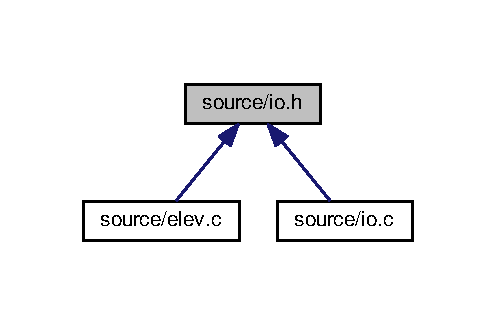
\includegraphics[width=238pt]{io_8h__dep__incl}
\end{center}
\end{figure}
\subsection*{Functions}
\begin{DoxyCompactItemize}
\item 
int \hyperlink{io_8h_a12ce98b64f2019ac45b44826a4db7ec9}{io\+\_\+init} ()
\item 
void \hyperlink{io_8h_a4d538858b80ee856217e3ecfde8a3c60}{io\+\_\+set\+\_\+bit} (int channel)
\item 
void \hyperlink{io_8h_a97951257634a0778b858a4ced7558f81}{io\+\_\+clear\+\_\+bit} (int channel)
\item 
void \hyperlink{io_8h_a1c2c5df63111187109ef11be354621bd}{io\+\_\+write\+\_\+analog} (int channel, int value)
\item 
int \hyperlink{io_8h_ae9e08ee7d41b07b153e2ddaae4dc53cb}{io\+\_\+read\+\_\+bit} (int channel)
\item 
int \hyperlink{io_8h_ab145a5637d2c463dfb5741e1a748dd74}{io\+\_\+read\+\_\+analog} (int channel)
\end{DoxyCompactItemize}


\subsection{Detailed Description}
IO module. 



\subsection{Function Documentation}
\index{io.\+h@{io.\+h}!io\+\_\+clear\+\_\+bit@{io\+\_\+clear\+\_\+bit}}
\index{io\+\_\+clear\+\_\+bit@{io\+\_\+clear\+\_\+bit}!io.\+h@{io.\+h}}
\subsubsection[{\texorpdfstring{io\+\_\+clear\+\_\+bit(int channel)}{io_clear_bit(int channel)}}]{\setlength{\rightskip}{0pt plus 5cm}void io\+\_\+clear\+\_\+bit (
\begin{DoxyParamCaption}
\item[{int}]{channel}
\end{DoxyParamCaption}
)}\hypertarget{io_8h_a97951257634a0778b858a4ced7558f81}{}\label{io_8h_a97951257634a0778b858a4ced7558f81}
Clears a digital channel bit. 
\begin{DoxyParams}{Parameters}
{\em channel} & Channel bit to set. \\
\hline
\end{DoxyParams}


Definition at line 45 of file io.\+c.

\index{io.\+h@{io.\+h}!io\+\_\+init@{io\+\_\+init}}
\index{io\+\_\+init@{io\+\_\+init}!io.\+h@{io.\+h}}
\subsubsection[{\texorpdfstring{io\+\_\+init()}{io_init()}}]{\setlength{\rightskip}{0pt plus 5cm}int io\+\_\+init (
\begin{DoxyParamCaption}
{}
\end{DoxyParamCaption}
)}\hypertarget{io_8h_a12ce98b64f2019ac45b44826a4db7ec9}{}\label{io_8h_a12ce98b64f2019ac45b44826a4db7ec9}
Initialize lib\+Comedi in \char`\"{}\+Sanntidssalen\char`\"{} \begin{DoxyReturn}{Returns}
Non-\/zero on success and 0 on failure 
\end{DoxyReturn}


Definition at line 18 of file io.\+c.

\index{io.\+h@{io.\+h}!io\+\_\+read\+\_\+analog@{io\+\_\+read\+\_\+analog}}
\index{io\+\_\+read\+\_\+analog@{io\+\_\+read\+\_\+analog}!io.\+h@{io.\+h}}
\subsubsection[{\texorpdfstring{io\+\_\+read\+\_\+analog(int channel)}{io_read_analog(int channel)}}]{\setlength{\rightskip}{0pt plus 5cm}int io\+\_\+read\+\_\+analog (
\begin{DoxyParamCaption}
\item[{int}]{channel}
\end{DoxyParamCaption}
)}\hypertarget{io_8h_ab145a5637d2c463dfb5741e1a748dd74}{}\label{io_8h_ab145a5637d2c463dfb5741e1a748dd74}
Reads a bit value from an analog channel. 
\begin{DoxyParams}{Parameters}
{\em channel} & Channel to read from. \\
\hline
\end{DoxyParams}
\begin{DoxyReturn}{Returns}
Value read. 
\end{DoxyReturn}


Definition at line 66 of file io.\+c.

\index{io.\+h@{io.\+h}!io\+\_\+read\+\_\+bit@{io\+\_\+read\+\_\+bit}}
\index{io\+\_\+read\+\_\+bit@{io\+\_\+read\+\_\+bit}!io.\+h@{io.\+h}}
\subsubsection[{\texorpdfstring{io\+\_\+read\+\_\+bit(int channel)}{io_read_bit(int channel)}}]{\setlength{\rightskip}{0pt plus 5cm}int io\+\_\+read\+\_\+bit (
\begin{DoxyParamCaption}
\item[{int}]{channel}
\end{DoxyParamCaption}
)}\hypertarget{io_8h_ae9e08ee7d41b07b153e2ddaae4dc53cb}{}\label{io_8h_ae9e08ee7d41b07b153e2ddaae4dc53cb}
Reads a bit value from a digital channel. 
\begin{DoxyParams}{Parameters}
{\em channel} & Channel to read from. \\
\hline
\end{DoxyParams}
\begin{DoxyReturn}{Returns}
Value read. 
\end{DoxyReturn}


Definition at line 57 of file io.\+c.

\index{io.\+h@{io.\+h}!io\+\_\+set\+\_\+bit@{io\+\_\+set\+\_\+bit}}
\index{io\+\_\+set\+\_\+bit@{io\+\_\+set\+\_\+bit}!io.\+h@{io.\+h}}
\subsubsection[{\texorpdfstring{io\+\_\+set\+\_\+bit(int channel)}{io_set_bit(int channel)}}]{\setlength{\rightskip}{0pt plus 5cm}void io\+\_\+set\+\_\+bit (
\begin{DoxyParamCaption}
\item[{int}]{channel}
\end{DoxyParamCaption}
)}\hypertarget{io_8h_a4d538858b80ee856217e3ecfde8a3c60}{}\label{io_8h_a4d538858b80ee856217e3ecfde8a3c60}
Sets a digital channel bit. 
\begin{DoxyParams}{Parameters}
{\em channel} & Channel bit to set. \\
\hline
\end{DoxyParams}


Definition at line 39 of file io.\+c.

\index{io.\+h@{io.\+h}!io\+\_\+write\+\_\+analog@{io\+\_\+write\+\_\+analog}}
\index{io\+\_\+write\+\_\+analog@{io\+\_\+write\+\_\+analog}!io.\+h@{io.\+h}}
\subsubsection[{\texorpdfstring{io\+\_\+write\+\_\+analog(int channel, int value)}{io_write_analog(int channel, int value)}}]{\setlength{\rightskip}{0pt plus 5cm}void io\+\_\+write\+\_\+analog (
\begin{DoxyParamCaption}
\item[{int}]{channel, }
\item[{int}]{value}
\end{DoxyParamCaption}
)}\hypertarget{io_8h_a1c2c5df63111187109ef11be354621bd}{}\label{io_8h_a1c2c5df63111187109ef11be354621bd}
Writes a value to an analog channel. 
\begin{DoxyParams}{Parameters}
{\em channel} & Channel to write to. \\
\hline
{\em value} & Value to write. \\
\hline
\end{DoxyParams}


Definition at line 51 of file io.\+c.


\hypertarget{main_8c}{}\section{source/main.c File Reference}
\label{main_8c}\index{source/main.\+c@{source/main.\+c}}


The main file, initializes elev, fsm and then runs the fsm.  


{\ttfamily \#include \char`\"{}elev.\+h\char`\"{}}\\*
{\ttfamily \#include \char`\"{}floor.\+h\char`\"{}}\\*
{\ttfamily \#include \char`\"{}F\+S\+M.\+h\char`\"{}}\\*
{\ttfamily \#include \char`\"{}door.\+h\char`\"{}}\\*
{\ttfamily \#include $<$stdio.\+h$>$}\\*
{\ttfamily \#include $<$time.\+h$>$}\\*
Include dependency graph for main.\+c\+:\nopagebreak
\begin{figure}[H]
\begin{center}
\leavevmode
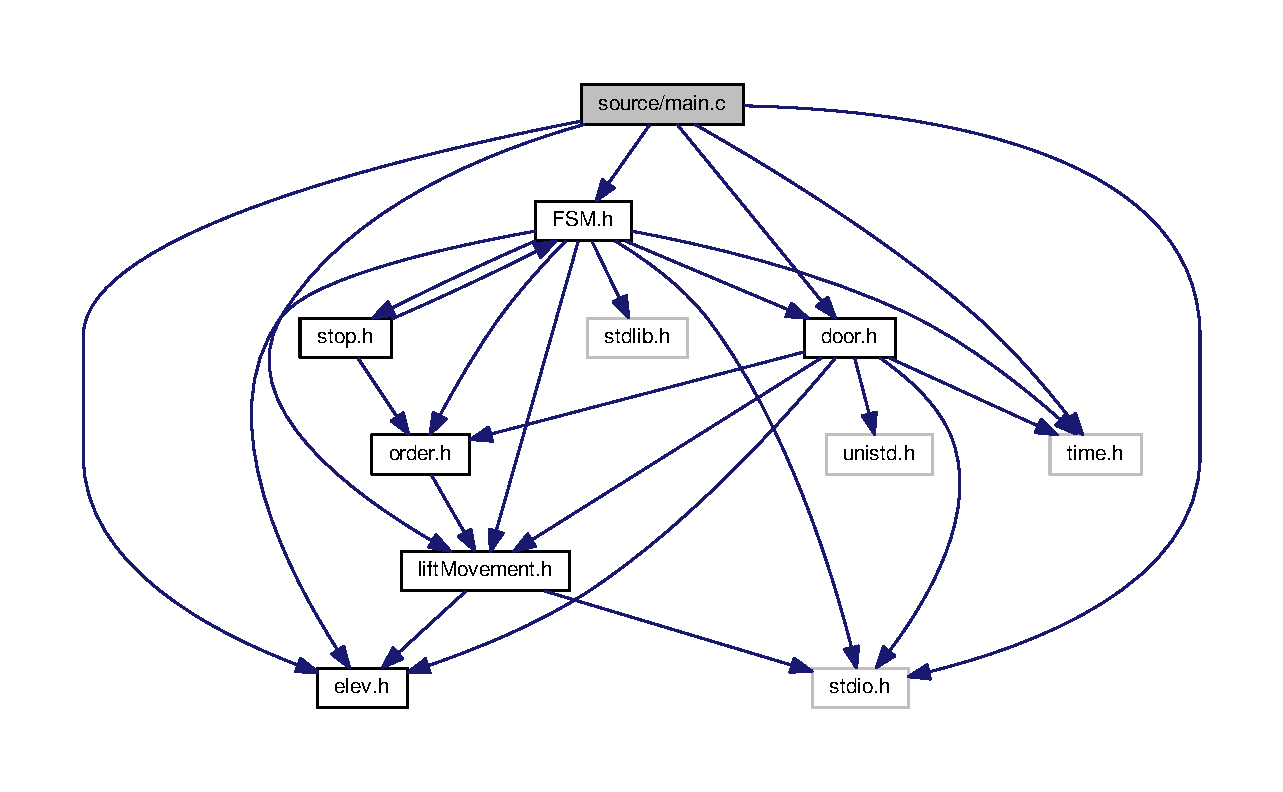
\includegraphics[width=350pt]{main_8c__incl}
\end{center}
\end{figure}
\subsection*{Functions}
\begin{DoxyCompactItemize}
\item 
int {\bfseries main} ()\hypertarget{main_8c_ae66f6b31b5ad750f1fe042a706a4e3d4}{}\label{main_8c_ae66f6b31b5ad750f1fe042a706a4e3d4}

\end{DoxyCompactItemize}


\subsection{Detailed Description}
The main file, initializes elev, fsm and then runs the fsm. 


\hypertarget{order_8h}{}\section{source/order.h File Reference}
\label{order_8h}\index{source/order.\+h@{source/order.\+h}}


Order module, stores the orders in two lists, checks for new orders, adds, removes and manages the orders by modifying these lists.  


{\ttfamily \#include \char`\"{}floor.\+h\char`\"{}}\\*
{\ttfamily \#include \char`\"{}F\+S\+M.\+h\char`\"{}}\\*
{\ttfamily \#include \char`\"{}elev.\+h\char`\"{}}\\*
{\ttfamily \#include $<$stdio.\+h$>$}\\*
Include dependency graph for order.\+h\+:\nopagebreak
\begin{figure}[H]
\begin{center}
\leavevmode
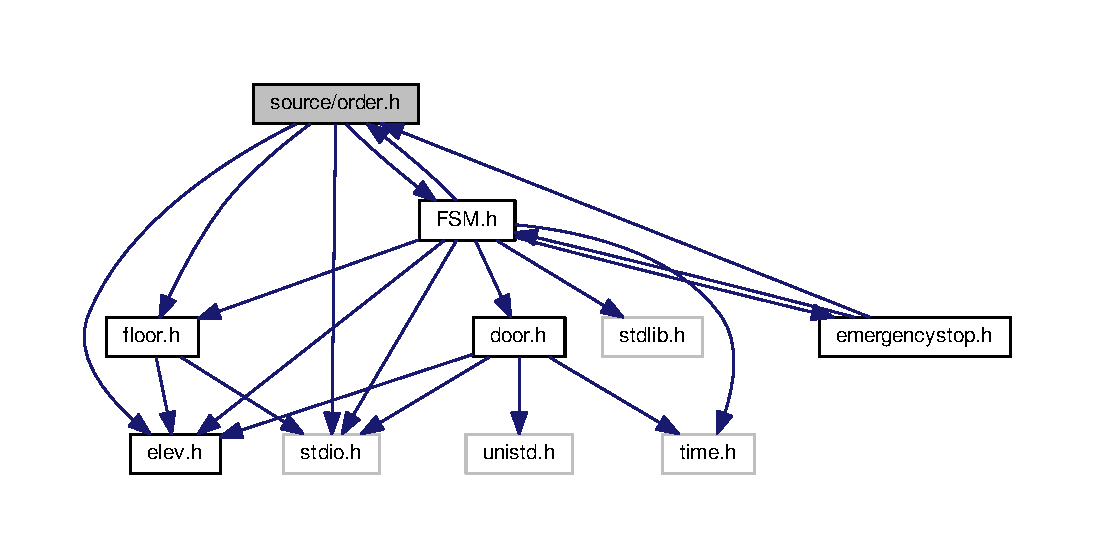
\includegraphics[width=350pt]{order_8h__incl}
\end{center}
\end{figure}
This graph shows which files directly or indirectly include this file\+:\nopagebreak
\begin{figure}[H]
\begin{center}
\leavevmode
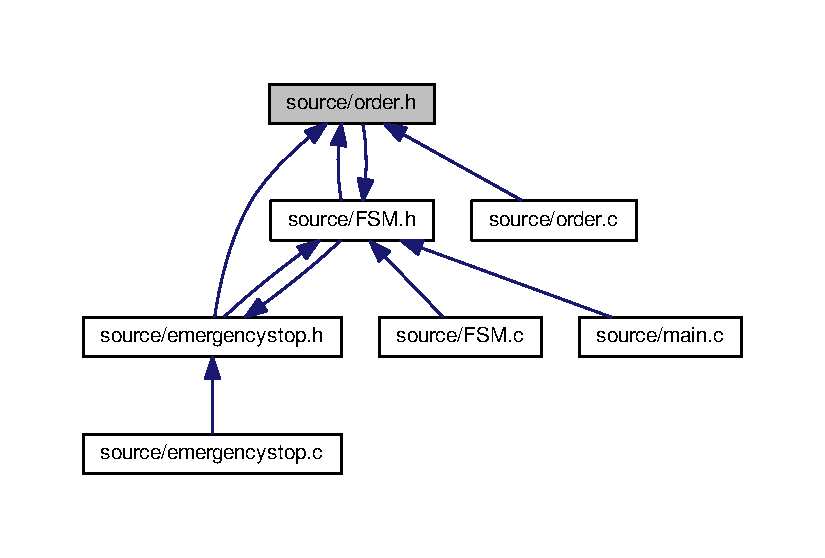
\includegraphics[width=350pt]{order_8h__dep__incl}
\end{center}
\end{figure}
\subsection*{Typedefs}
\begin{DoxyCompactItemize}
\item 
typedef enum \hyperlink{order_8h_af70dc8a017aa38cddee7df9ea775bff6}{tag\+\_\+order\+\_\+type} \hyperlink{order_8h_ad3b024fcdc8bf8e7a363526f7cbcef1c}{order\+\_\+type\+\_\+t}
\end{DoxyCompactItemize}
\subsection*{Enumerations}
\begin{DoxyCompactItemize}
\item 
enum \hyperlink{order_8h_af70dc8a017aa38cddee7df9ea775bff6}{tag\+\_\+order\+\_\+type} \{ {\bfseries D\+O\+WN} = -\/1, 
{\bfseries C\+O\+M\+M\+A\+ND}, 
{\bfseries UP}
 \}
\end{DoxyCompactItemize}
\subsection*{Functions}
\begin{DoxyCompactItemize}
\item 
void \hyperlink{order_8h_aa679e940f2ab0cdcd1734e9dd59edbbf}{print\+\_\+order} ()
\item 
void \hyperlink{order_8h_ae2a981fdadfc41c09b6d303dc7502d29}{add\+Order\+\_\+order} (\hyperlink{floor_8h_acb30631293fda569568eff832f5185b4}{Floor} floor, \hyperlink{order_8h_ad3b024fcdc8bf8e7a363526f7cbcef1c}{order\+\_\+type\+\_\+t} order\+\_\+type)
\item 
void \hyperlink{order_8h_a7871cdd48140558f433475a8a137311e}{remove\+Orders\+\_\+order} (\hyperlink{floor_8h_acb30631293fda569568eff832f5185b4}{Floor} floor)
\item 
void \hyperlink{order_8h_a725fed933533852b6c14974f96032ea0}{check\+For\+Orders\+\_\+order} ()
\item 
\hyperlink{elev_8h_a2256dfd58fecce253106f83fd2ed607f}{elev\+\_\+motor\+\_\+direction\+\_\+t} \hyperlink{order_8h_a971e3a926a57ef7a94bb166d76043e6d}{select\+Dir\+\_\+order} (float inbetween\+\_\+floor, \hyperlink{elev_8h_a2256dfd58fecce253106f83fd2ed607f}{elev\+\_\+motor\+\_\+direction\+\_\+t} current\+\_\+direction)
\item 
void \hyperlink{order_8h_a06ee0e7888023fb4619b7802bbcb40af}{remove\+All\+Orders\+\_\+order} ()
\item 
int \hyperlink{order_8h_af2019f6b13b136e72d60311f355c11f9}{is\+Order\+In\+Floor\+\_\+order} (\hyperlink{floor_8h_acb30631293fda569568eff832f5185b4}{Floor} floor)
\item 
int \hyperlink{order_8h_a14bf4c53b56a07e544dd4fde3979dbaf}{should\+Lift\+Stop\+\_\+order} (\hyperlink{floor_8h_acb30631293fda569568eff832f5185b4}{Floor} floor, \hyperlink{elev_8h_a2256dfd58fecce253106f83fd2ed607f}{elev\+\_\+motor\+\_\+direction\+\_\+t} motor\+\_\+dir\+\_\+g)
\item 
int \hyperlink{order_8h_a5341996224daa682d522c4a1b7f782d7}{are\+Order\+Lists\+Empty\+\_\+order} ()
\end{DoxyCompactItemize}


\subsection{Detailed Description}
Order module, stores the orders in two lists, checks for new orders, adds, removes and manages the orders by modifying these lists. 



\subsection{Typedef Documentation}
\index{order.\+h@{order.\+h}!order\+\_\+type\+\_\+t@{order\+\_\+type\+\_\+t}}
\index{order\+\_\+type\+\_\+t@{order\+\_\+type\+\_\+t}!order.\+h@{order.\+h}}
\subsubsection[{\texorpdfstring{order\+\_\+type\+\_\+t}{order_type_t}}]{\setlength{\rightskip}{0pt plus 5cm}typedef enum {\bf tag\+\_\+order\+\_\+type}  {\bf order\+\_\+type\+\_\+t}}\hypertarget{order_8h_ad3b024fcdc8bf8e7a363526f7cbcef1c}{}\label{order_8h_ad3b024fcdc8bf8e7a363526f7cbcef1c}
Which order button type we have. Can be {\ttfamily D\+O\+WN} (outside lift down button), {\ttfamily C\+O\+M\+M\+A\+ND} (inside lift any button) or {\ttfamily UP} (outside lift up button). 

\subsection{Enumeration Type Documentation}
\index{order.\+h@{order.\+h}!tag\+\_\+order\+\_\+type@{tag\+\_\+order\+\_\+type}}
\index{tag\+\_\+order\+\_\+type@{tag\+\_\+order\+\_\+type}!order.\+h@{order.\+h}}
\subsubsection[{\texorpdfstring{tag\+\_\+order\+\_\+type}{tag_order_type}}]{\setlength{\rightskip}{0pt plus 5cm}enum {\bf tag\+\_\+order\+\_\+type}}\hypertarget{order_8h_af70dc8a017aa38cddee7df9ea775bff6}{}\label{order_8h_af70dc8a017aa38cddee7df9ea775bff6}
Which order button type we have. Can be {\ttfamily D\+O\+WN} (outside lift down button), {\ttfamily C\+O\+M\+M\+A\+ND} (inside lift any button) or {\ttfamily UP} (outside lift up button). 

Definition at line 18 of file order.\+h.



\subsection{Function Documentation}
\index{order.\+h@{order.\+h}!add\+Order\+\_\+order@{add\+Order\+\_\+order}}
\index{add\+Order\+\_\+order@{add\+Order\+\_\+order}!order.\+h@{order.\+h}}
\subsubsection[{\texorpdfstring{add\+Order\+\_\+order(\+Floor floor, order\+\_\+type\+\_\+t order\+\_\+type)}{addOrder_order(Floor floor, order_type_t order_type)}}]{\setlength{\rightskip}{0pt plus 5cm}void add\+Order\+\_\+order (
\begin{DoxyParamCaption}
\item[{{\bf Floor}}]{floor, }
\item[{{\bf order\+\_\+type\+\_\+t}}]{order\+\_\+type}
\end{DoxyParamCaption}
)}\hypertarget{order_8h_ae2a981fdadfc41c09b6d303dc7502d29}{}\label{order_8h_ae2a981fdadfc41c09b6d303dc7502d29}
Add an order to one/both of the {\ttfamily order} lists 
\begin{DoxyParams}{Parameters}
{\em order\+\_\+type} & Which order button type we have. Can be {\ttfamily D\+O\+WN} (outside lift down button), {\ttfamily C\+O\+M\+M\+A\+ND} (inside lift any button) or {\ttfamily UP} (outside lift up button). \\
\hline
{\em floor} & Which floor the lift is ordered to go to. Must be 0-\/3. \\
\hline
\end{DoxyParams}


Definition at line 16 of file order.\+c.

\index{order.\+h@{order.\+h}!are\+Order\+Lists\+Empty\+\_\+order@{are\+Order\+Lists\+Empty\+\_\+order}}
\index{are\+Order\+Lists\+Empty\+\_\+order@{are\+Order\+Lists\+Empty\+\_\+order}!order.\+h@{order.\+h}}
\subsubsection[{\texorpdfstring{are\+Order\+Lists\+Empty\+\_\+order()}{areOrderListsEmpty_order()}}]{\setlength{\rightskip}{0pt plus 5cm}int are\+Order\+Lists\+Empty\+\_\+order (
\begin{DoxyParamCaption}
{}
\end{DoxyParamCaption}
)}\hypertarget{order_8h_a5341996224daa682d522c4a1b7f782d7}{}\label{order_8h_a5341996224daa682d522c4a1b7f782d7}
Checks if order lists are empty \begin{DoxyReturn}{Returns}
1 if there are any orders, 0 if there are no orders. 
\end{DoxyReturn}


Definition at line 115 of file order.\+c.

\index{order.\+h@{order.\+h}!check\+For\+Orders\+\_\+order@{check\+For\+Orders\+\_\+order}}
\index{check\+For\+Orders\+\_\+order@{check\+For\+Orders\+\_\+order}!order.\+h@{order.\+h}}
\subsubsection[{\texorpdfstring{check\+For\+Orders\+\_\+order()}{checkForOrders_order()}}]{\setlength{\rightskip}{0pt plus 5cm}void check\+For\+Orders\+\_\+order (
\begin{DoxyParamCaption}
{}
\end{DoxyParamCaption}
)}\hypertarget{order_8h_a725fed933533852b6c14974f96032ea0}{}\label{order_8h_a725fed933533852b6c14974f96032ea0}
Checks for incoming orders and adds them to lists (by calling add\+Order function) 

Definition at line 49 of file order.\+c.

\index{order.\+h@{order.\+h}!is\+Order\+In\+Floor\+\_\+order@{is\+Order\+In\+Floor\+\_\+order}}
\index{is\+Order\+In\+Floor\+\_\+order@{is\+Order\+In\+Floor\+\_\+order}!order.\+h@{order.\+h}}
\subsubsection[{\texorpdfstring{is\+Order\+In\+Floor\+\_\+order(\+Floor floor)}{isOrderInFloor_order(Floor floor)}}]{\setlength{\rightskip}{0pt plus 5cm}int is\+Order\+In\+Floor\+\_\+order (
\begin{DoxyParamCaption}
\item[{{\bf Floor}}]{floor}
\end{DoxyParamCaption}
)}\hypertarget{order_8h_af2019f6b13b136e72d60311f355c11f9}{}\label{order_8h_af2019f6b13b136e72d60311f355c11f9}

\begin{DoxyParams}{Parameters}
{\em floor} & Which floor to check for orders \\
\hline
\end{DoxyParams}
\begin{DoxyReturn}{Returns}
1 if there is an order i floor, 0 if there are none. 
\end{DoxyReturn}


Definition at line 180 of file order.\+c.

\index{order.\+h@{order.\+h}!print\+\_\+order@{print\+\_\+order}}
\index{print\+\_\+order@{print\+\_\+order}!order.\+h@{order.\+h}}
\subsubsection[{\texorpdfstring{print\+\_\+order()}{print_order()}}]{\setlength{\rightskip}{0pt plus 5cm}void print\+\_\+order (
\begin{DoxyParamCaption}
{}
\end{DoxyParamCaption}
)}\hypertarget{order_8h_aa679e940f2ab0cdcd1734e9dd59edbbf}{}\label{order_8h_aa679e940f2ab0cdcd1734e9dd59edbbf}
Prints our current pending orders. 

Definition at line 4 of file order.\+c.

\index{order.\+h@{order.\+h}!remove\+All\+Orders\+\_\+order@{remove\+All\+Orders\+\_\+order}}
\index{remove\+All\+Orders\+\_\+order@{remove\+All\+Orders\+\_\+order}!order.\+h@{order.\+h}}
\subsubsection[{\texorpdfstring{remove\+All\+Orders\+\_\+order()}{removeAllOrders_order()}}]{\setlength{\rightskip}{0pt plus 5cm}void remove\+All\+Orders\+\_\+order (
\begin{DoxyParamCaption}
{}
\end{DoxyParamCaption}
)}\hypertarget{order_8h_a06ee0e7888023fb4619b7802bbcb40af}{}\label{order_8h_a06ee0e7888023fb4619b7802bbcb40af}
Removes all orders. 

Definition at line 125 of file order.\+c.

\index{order.\+h@{order.\+h}!remove\+Orders\+\_\+order@{remove\+Orders\+\_\+order}}
\index{remove\+Orders\+\_\+order@{remove\+Orders\+\_\+order}!order.\+h@{order.\+h}}
\subsubsection[{\texorpdfstring{remove\+Orders\+\_\+order(\+Floor floor)}{removeOrders_order(Floor floor)}}]{\setlength{\rightskip}{0pt plus 5cm}void remove\+Orders\+\_\+order (
\begin{DoxyParamCaption}
\item[{{\bf Floor}}]{floor}
\end{DoxyParamCaption}
)}\hypertarget{order_8h_a7871cdd48140558f433475a8a137311e}{}\label{order_8h_a7871cdd48140558f433475a8a137311e}
Removes all order in inputed floor, and turns off corresponding order button lights 
\begin{DoxyParams}{Parameters}
{\em floor} & Which floor to remove order in. Must be 0-\/3. \\
\hline
\end{DoxyParams}


Definition at line 33 of file order.\+c.

\index{order.\+h@{order.\+h}!select\+Dir\+\_\+order@{select\+Dir\+\_\+order}}
\index{select\+Dir\+\_\+order@{select\+Dir\+\_\+order}!order.\+h@{order.\+h}}
\subsubsection[{\texorpdfstring{select\+Dir\+\_\+order(float inbetween\+\_\+floor, elev\+\_\+motor\+\_\+direction\+\_\+t current\+\_\+direction)}{selectDir_order(float inbetween_floor, elev_motor_direction_t current_direction)}}]{\setlength{\rightskip}{0pt plus 5cm}{\bf elev\+\_\+motor\+\_\+direction\+\_\+t} select\+Dir\+\_\+order (
\begin{DoxyParamCaption}
\item[{float}]{inbetween\+\_\+floor, }
\item[{{\bf elev\+\_\+motor\+\_\+direction\+\_\+t}}]{current\+\_\+direction}
\end{DoxyParamCaption}
)}\hypertarget{order_8h_a971e3a926a57ef7a94bb166d76043e6d}{}\label{order_8h_a971e3a926a57ef7a94bb166d76043e6d}
Selects which direction the elevator should move. \begin{DoxyReturn}{Returns}
a {\ttfamily elev\+\_\+motor\+\_\+direction\+\_\+t} which can be {\ttfamily D\+I\+R\+N\+\_\+\+D\+O\+WN}, {\ttfamily D\+I\+R\+N\+\_\+\+S\+T\+OP} or {\ttfamily D\+I\+R\+N\+\_\+\+UP}. 
\end{DoxyReturn}


Definition at line 64 of file order.\+c.

\index{order.\+h@{order.\+h}!should\+Lift\+Stop\+\_\+order@{should\+Lift\+Stop\+\_\+order}}
\index{should\+Lift\+Stop\+\_\+order@{should\+Lift\+Stop\+\_\+order}!order.\+h@{order.\+h}}
\subsubsection[{\texorpdfstring{should\+Lift\+Stop\+\_\+order(\+Floor floor, elev\+\_\+motor\+\_\+direction\+\_\+t motor\+\_\+dir\+\_\+g)}{shouldLiftStop_order(Floor floor, elev_motor_direction_t motor_dir_g)}}]{\setlength{\rightskip}{0pt plus 5cm}int should\+Lift\+Stop\+\_\+order (
\begin{DoxyParamCaption}
\item[{{\bf Floor}}]{floor, }
\item[{{\bf elev\+\_\+motor\+\_\+direction\+\_\+t}}]{motor\+\_\+dir\+\_\+g}
\end{DoxyParamCaption}
)}\hypertarget{order_8h_a14bf4c53b56a07e544dd4fde3979dbaf}{}\label{order_8h_a14bf4c53b56a07e544dd4fde3979dbaf}

\begin{DoxyParams}{Parameters}
{\em floor} & The floor the lift should consider stopping in. \\
\hline
{\em motor\+\_\+dir} & The direction the lift is currently moving in. \\
\hline
\end{DoxyParams}
\begin{DoxyReturn}{Returns}
1 if the lift should stop, 0 if the lift shouldnt stop. 
\end{DoxyReturn}


Definition at line 141 of file order.\+c.


%--- End generated contents ---

% Index
\backmatter
\newpage
\phantomsection
\clearemptydoublepage
\addcontentsline{toc}{chapter}{Index}
\printindex

\end{document}
